\documentclass[conference, a4paper]{IEEEtran}
\IEEEoverridecommandlockouts
% The preceding line is only needed to identify funding in the first footnote. If that is unneeded, please comment it out.
\usepackage{cite}
\usepackage{amsmath,amssymb,amsfonts}
\usepackage{algorithmic}
\usepackage{graphicx}
\usepackage{textcomp}
\usepackage{xcolor}
\def\BibTeX{{\rm B\kern-.05em{\sc i\kern-.025em b}\kern-.08em
    T\kern-.1667em\lower.7ex\hbox{E}\kern-.125emX}}
\ifCLASSOPTIONcompsoc
    \usepackage[caption=false, font=normalsize, labelfont=sf, textfont=sf]{subfig}
\else
\usepackage[caption=false, font=footnotesize]{subfig}
\fi

\addtolength{\topmargin}{+0.12cm}

\columnsep 0.25in

\begin{document}

\title{Wheat Yield Forecasting using Regression Algorithms and Neural Network}
\author{\IEEEauthorblockN{ Cheng Dai}
\IEEEauthorblockA{\textit{School of Information and Communication Engineering } \\
\textit{University of Electronic Science and Technology of China}\\
Chengdu, China \\
daichengzyw@gmail.com}
\and
\IEEEauthorblockN{Yinqin Huang}
\IEEEauthorblockA{\textit{School of Information and Communication Engineering,} \\
\textit{University of Electronic Science and Technology of China}\\
Chengdu, China  \\
hyinq@hotmail.com}
\and
\IEEEauthorblockN{Minghao Ni}
\IEEEauthorblockA{\textit{School of Information and Communication Engineering} \\
\textit{University of Electronic Science and Technology of China}\\
Chengdu, China \\
845101809@qq.com}
\and
\IEEEauthorblockN{Xingang Liu*}
\IEEEauthorblockA{\textit{School of Information and Communication Engineering} \\
\textit{University of Electronic Science and Technology of China}\\
Chengdu, China \\
hanksliu@uestc.edu.cn}
}

\maketitle

\begin{abstract}
<<<<<<< HEAD
  The demand for food 
  This paper considers the crop yield forecasting problem base on the wheat yield dataset of the U.S. To provide advice for farmers to raise the per-unit-area yield under the circumstance that the demand for food production is significantly increasing while the cultivated land area haven't expanded in recent decades, we composed a Bi-LSTM model with convolutional neural networks feature extraction sub-network to predict the wheat yield. The results of the experiment show that the model outperforms the other regression algorithms we have tested on the same dataset and can overcome the overfitting problem which is commonly found in other algorithms. The $R^2$ score of the model reaches 0.87 and the MSE is 19.6252. 
=======
  % This paper considers the crop yield forecasting problem base on the wheat yield dataset of the U.S. To provide advice for farmers to raise the per unit area yield under the circumstance that the demand for food production are significantly increasing while the cultivated land area not expanded in recent decades, we compose a Bi-LSTM model consists of 3 stacked Bi-LSTM layers to predict wheat yield and test common used regression algorithms on the same dataset which have been preprocessed including the processing of filling in the missing items, dropping abnormal data and feature selection. The result shows that the Bi-LSTM model's $R^2$ score is 0.85 which outperforms the other algorithms. This model can also avoid overfitting problem which is commonly found in other regression algorithms. 
  This paper considers the crop yield forecasting problem base on the wheat yield dataset of the U.S. To provide advice for farmers to raise the per-unit-area yield under the circumstance that the demand for food production is significantly increasing while the cultivated land area haven't expanded in recent decades, we composed a Bi-LSTM model with convolutional neural networks feature extraction sub-network to predict the wheat yield. The results of the experiment show that the model outperforms the other regression algorithms we have tested on the same dataset and can overcome the overfitting problem which is commonly found in other algorithms. The $R^2$ score of the model reaches 0.84 and the MSE is 12.37. 
>>>>>>> 3f857d160bf9233a059c88a168185e20cc1bc003
  % TODO: 最终的结果需要检查
\end{abstract}

\begin{IEEEkeywords}
  Prediction, Agricultural Yield, Random Forest, LSTM RNN
\end{IEEEkeywords}

\section{Introduction}
  The food issue has always been a hot topic and directly affects many aspects of people's lives. With the explosive growth of the world population, countries all over the world are exploring methods to grow crops with less natural resource consumption while increasing production under the guarantee of environmental protection. In such situation, the precision and intelligence of agriculture are becoming increasingly important. Therefore, researchers have focused on the collection, combination and processing of external information including data of climate, satellites and geography in recent years. Such researches do improved the modern agricultural technology and also helped increase agricultural yield and crop quality.\par
  The forecast of crop yield is an important part of modern agricultural technology, which can help people adjust cultivate methods in time and improve production efficiency. Many developed countries and regions have developed advanced agricultural yield forecasting system, such as Monitoring Agricultural Resources (MARS) of EU\cite{vanderveldePerformanceMARScropYield2019}. MARS has been using remote sensing since 1988, which initially designed to apply the newly emerging space technologies for providing independent and timely information on crop areas and yields, and has become a integrated system of agricultural monitoring and forecast.\par
  Over the past few decades, regression algorithms and sensor technologies have developed rapidly with the advancement of computing hardware and theories, that development directly leads to the emergence of more accurate algorithms of prediction. At the beginning, statistical-based models with probability theory or regression methods were widely used to implement yield forecasting\cite{matisMarkovChainApproach1985, stephensCropYieldForecasting1995}. Since the explosive development of space technology and electronic industry, remote sensing and sensor network are employed to farmland monitoring.  The data from remote sensing and sensor network have played an important role in the improvement of the prediction accuracy\cite{youDeepGaussianProcess2017, baruthUseRemoteSensing}. Recent years, the raise of deep learning has also boosted the development of crop yield forecasting. Many deep learning models have been applied to this area, which allows more complicated data, such as genetic information, to be processed comparing to the statistical weather data\cite{mateo-sanchisSynergisticIntegrationOptical2019,steenUsingDeepLearning2016a}. Another advantage of deep learning is the feature extraction, that data from higher levels of the hierarchy are formed by the composition of lower level features\cite{lecunDeepLearning2015}.\par
  In this paper, we proposed a Bi-LSTM model with CNN feature extraction sub-network to predict the yield on a dataset including weather data and wheat yield from 1895 different plant locations of the U.S in 2013 and 2014. The rest of this paper is organized as follows. Section.\ref{sec:RW} introduces the common used methods in crop yield prediction. Section.\ref{sec:MB} introduces the mathematic backgrounds of the LSTM and the bidirectional RNN, Section.\ref{sec:Arch} introduces the architecture of the Bi-LSTM model and in Section.\ref{sec:ex} experiment results are revealed and we discuss its feasibility and advantages. Finally, the conclusion and some directions of future work are given about our method in Section.\ref{sec:con}.

\section{Related works} \label{sec:RW}

  The most common models which has been used for decades to forecast the crop yield are statistical-based models. Such methods feed agrometeorological data to a regression model, and finally are in the form of a function whose independent variables are agrometeorological parameters such as precipitation and temperature. The simplicity of regression models results in the applicability in crop yield forecasting. On the contrary, the limitations of data sources and observation boundaries make it hardly to extrapolate results to other locations. USDA (2011) \cite{goodUSDACornSoybean2011} have been using such statistical-based regression model to forecast yield of corn in 10 major corn-producing countries for years. Tack (2015)\cite{tackEffectWarmingTemperatures2015} used a quadratic regression model base on the weather data and wheat yield of Kansas during 1985 to 2013 to research on how the temperature effects the wheat yield during the growing season in the context of global warming, the result shows that the largest factor of yield loss are freezing temperatures in the Fall and extreme heat events in the Spring, they also found that the overall rising temperature imposes negative influence on wheat yield even after accounting for the benefits of reduced exposure to freezing temperatures. 

  Recently, given the increasing amount of climate parameters collected by sensors with evolving performance, data which is more accurate to explain the crop condition like biomass and growth stage have been added into the models. Giri (2017) \cite{giriDistrictwiseWheatRice2017} developed a district-wise regression model to predict the wheat and rice yield in seven districts of eastern Madhya Pradesh India using combined climatic data and agrometeorological data. Their experiment result shows that the deviation between reported and forecasted yield was less than 15 percent. Singh (2017) \cite{singhForecastingMaizeYield2017} went a step further, they calculated two derivative variables for each weather variable, one as simple accumulation of weather variable and the other one as weighted accumulation of weekly data on weather variable. Then they train the model separately in different districts, and the $R^2$ score varies from 0.32 to 0.88 in different districts. Schauberger(2017)\cite{schaubergerGlobalEvaluationSemiempirical2017} concentrate on detecting weather influence on yield anomalies and project yields with unknown weather, they build an ordinary least squares regression scheme based on the Cobb-Douglas production function with different model specifications and their model can explain 63\%-81\% of observed yield anomalies of the US in the experiment.

  Except for naive statistical-based regression algorithms, advanced machine learning techniques also have been used in this area. Sisodia et al. (2018) \cite{sisodiaPreharvestForecastModel2018} build a multiple linear regression model with discriminant function analysis to predict the rice yield base on biometric characters. The experiment result has shown that the percent standard errors of prediction with real records is below 5\%. Mokarram and Bjianzadeh (2016) \cite{mokarramPredictionBiologicalGrain2016} compare and analyze the multiple linear regression and fully connected neural network with one hidden layer of predicting yield of barely, their experiments have proved that neural network models outperform the naive regression models with the same data inputs. 

  With GPU getting involved to boost the computing neural network training procedure, an increasing number of researchers have focused on deep learning algorithms which allow to input more complicated data to get more accurate forecasting results. Basso(2013)\cite{bassoReviewCropYield2013} uses deep neural networks to predict the maize yield with a dataset containing 2267 hybrids planted in 2247 locations between 2008 and 2016. Their DNN model has a superior prediction accuracy, with 12\% root-mean-square-error (RMSE) and 50\% standard deviation of the average yield on validation datasets. You(2017)\cite{youDeepGaussianProcess2017} proposed a dimensionality reduction technique based on CNN or LSTM, which can automatically learn features with scarce labeled data. This algorithm incorporates a Gaussian Process component to explicitly model the spatial-temporal structure of the data and improves accuracy on the prediction of soybean yield. The experimental results verify that this model outperforms state-of-the-art algorithms. Elavarasan and Vincent (2020) \cite{elavarasanCropYieldPrediction2020} propose a deep recurrent Q-network model with the construction of a recurrent neural network over the Q-Learning reinforcement learning algorithm, and the prediction accuracy on the original data distribution is 93.7\%.


\section{Mathematic backgrounds} \label{sec:MB}
  Since The Bi-LSTM structure is employed to predict the yield, some mathematic backgrounds about LSTM and Bidirectional wrapper will be introduced in this part.
  \subsection{LSTM Node}
    Recurrent Neural Network is a kind of neural network that is good at processing time-series data. It can well process tasks with continuous-time and contextual relationships which is exactly in line with the characteristics of the crop growth. The connections existing between each layer make the network better in learning time series relations, but on the other hand, this leads to a gradient explosion in backpropagation \cite{hochreiterLongShorttermMemory1997}.

    \begin{figure}[htbp]
      \centerline{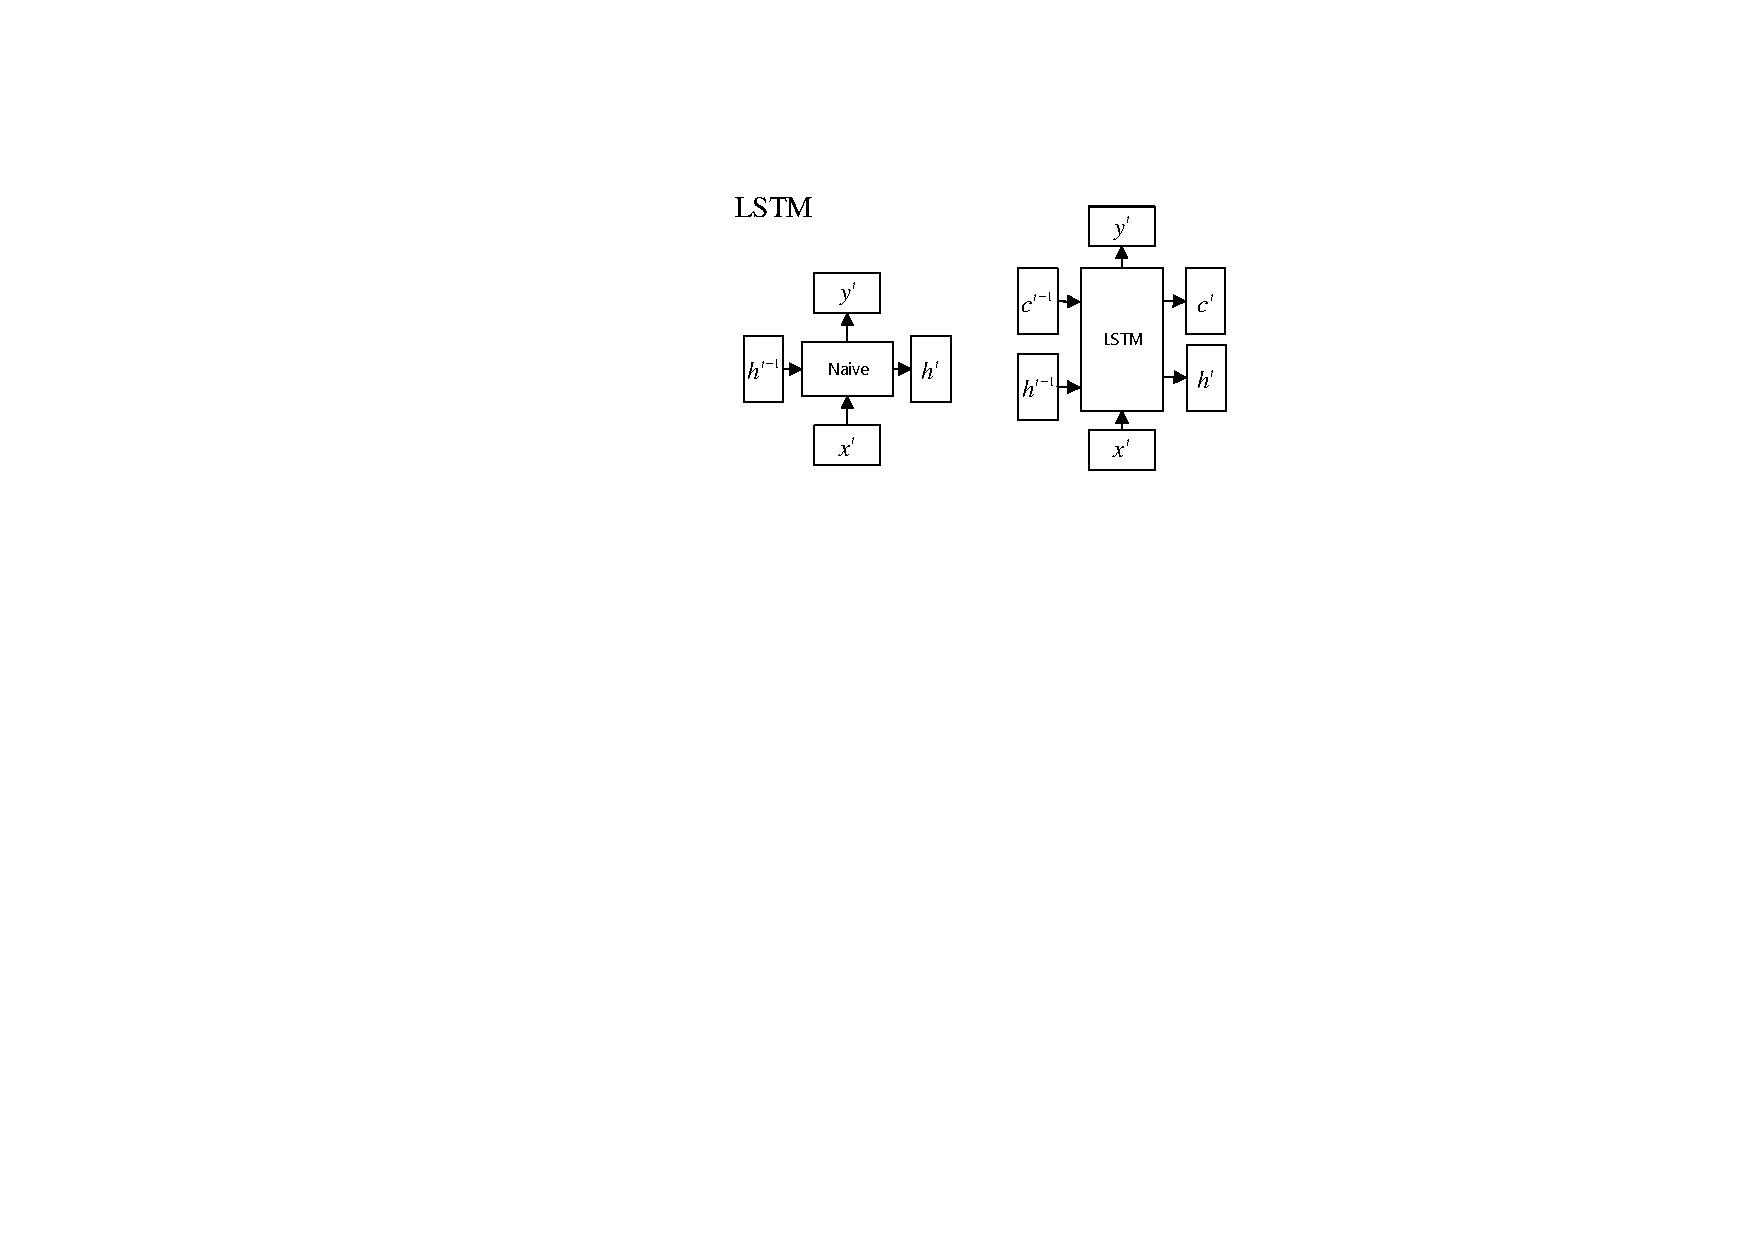
\includegraphics[width=0.7\linewidth]{figures/LSTM_struc.pdf}}
      \caption{LSTM and RNN structure}
      \label{fig:LSTM}
    \end{figure}

    Fig.~\ref{fig:LSTM} shows the structure of LSTM and RNN. The structure of t-th RNN node on the first image, where $x^t$ is the input of t-th node, $h^{t-1}$ is the input of t-th node received from $t-1$th node, $y^t$ is the output and $h^t$ is the output which will transfer to next node. The structure of t-th LSTM node is shown on the second image, that structure have two more states $c^t$(cell state) and $h^t$(hidden state), state $c$ in LSTM is the counterpart of state $h$ in RNN, and normally state $c$ changes slowly in front propagation and add a number to $c^{t-1}$ while $h^t$ changes drastically.

    \begin{figure}[htbp]
      \centerline{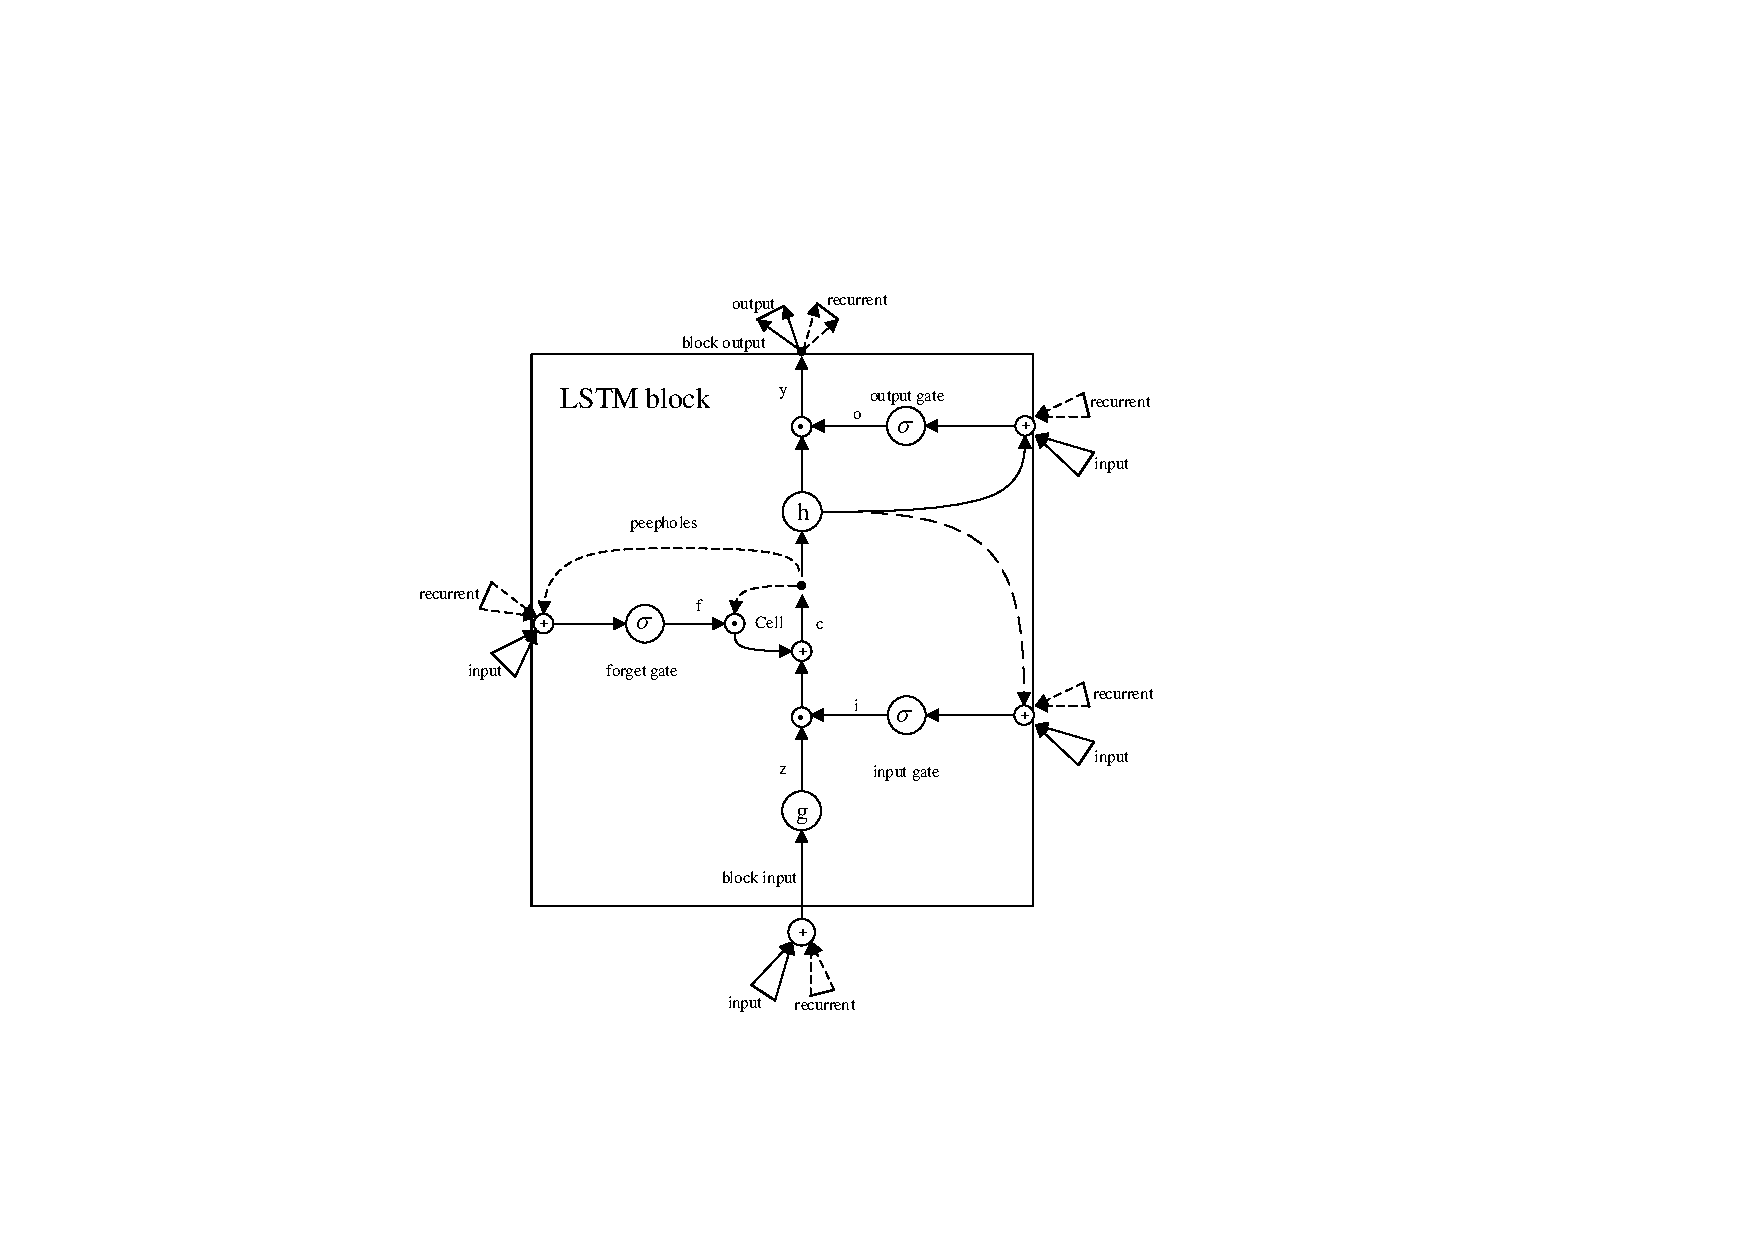
\includegraphics[width=0.7\linewidth]{figures/LSTM_node.pdf}}
      \caption{LSTM node}
      \label{fig:LSTM2}
    \end{figure}

    \begin{equation}
      \begin{cases}	f_t=\sigma \left( w_f\cdot \left[ h_{t-1},x_t \right] +b_f \right)\\	i_t=\sigma \left( w_i\cdot \left[ h_{t-1},x_t \right] +b_i \right)\\	o_t=\sigma \left( w_o\cdot \left[ h_{t-1},x_t \right] +b_i \right)\\\end{cases}
      \label{eq:gate}
    \end{equation}

    \begin{equation}
      \sigma \left( x \right) =\frac{1}{1+e^{-x}}
      \label{eq:sigmoid}
    \end{equation}

    For a LSTM node shown in Fig.~\ref{fig:LSTM2}, four states $f_t$(forget gate), $i_t$(input gate), $c_t$(current state) and $o_t$(output gate) are generated by concating $x^t$ and $h^{t-1}$ via (\ref{eq:gate}). Forget gate $f_t$ controls the remaining of information transferred from $c_{t-1}$, and $[h_{t-1}, x_t]$ means to concat vector $h_{t-1}$ and vector $x_t$. $w_f$ and $b_f$ are the weight and bias of forget gate $f_t$, $\sigma$ is the Sigmoid activation function whose expression is (\ref{eq:sigmoid}).

    To calculate $c_t$, the input state $\widetilde{c_t}$ are needed. Use activation function $\tanh$ and (\ref{eq:ct1}), (\ref{eq:ct2}) and (\ref{eq:gate}) to calculate $c_t$, the $\odot$ in (\ref{eq:ct2}) means corresponding element multiplication.

    \begin{equation}
      \tilde{c}_t=\tanh \left( W_c\cdot \left[ h_{t-q},x_t \right] +b_c \right)
      \label{eq:ct1}
    \end{equation}

    \begin{equation}
      c_t=f_t\odot c_{t-1}+i_t\odot c_t
      \label{eq:ct2}
    \end{equation}

    All these features of LSTM meet the crop growing process, there are weather fluctuations or natural disasters in a short time, while there are stable natural conditions over a long period.

  \subsection{Bidirectional RNN}
    Mike Schuster \cite{schusterBidirectionalRecurrentNeural1997} proposed the Bi-directional RNN(BRNN) in 1997 as shown in Fig.~\ref{fig:BRNN}. In his paper, the conventional RNN neurons are splited into two parts, one for negative time direction and the other for positive time direction. The output of the forward states will not be send to the backward states. 
    % TODO: 再写点

    \begin{figure}[htbp]
      \centerline{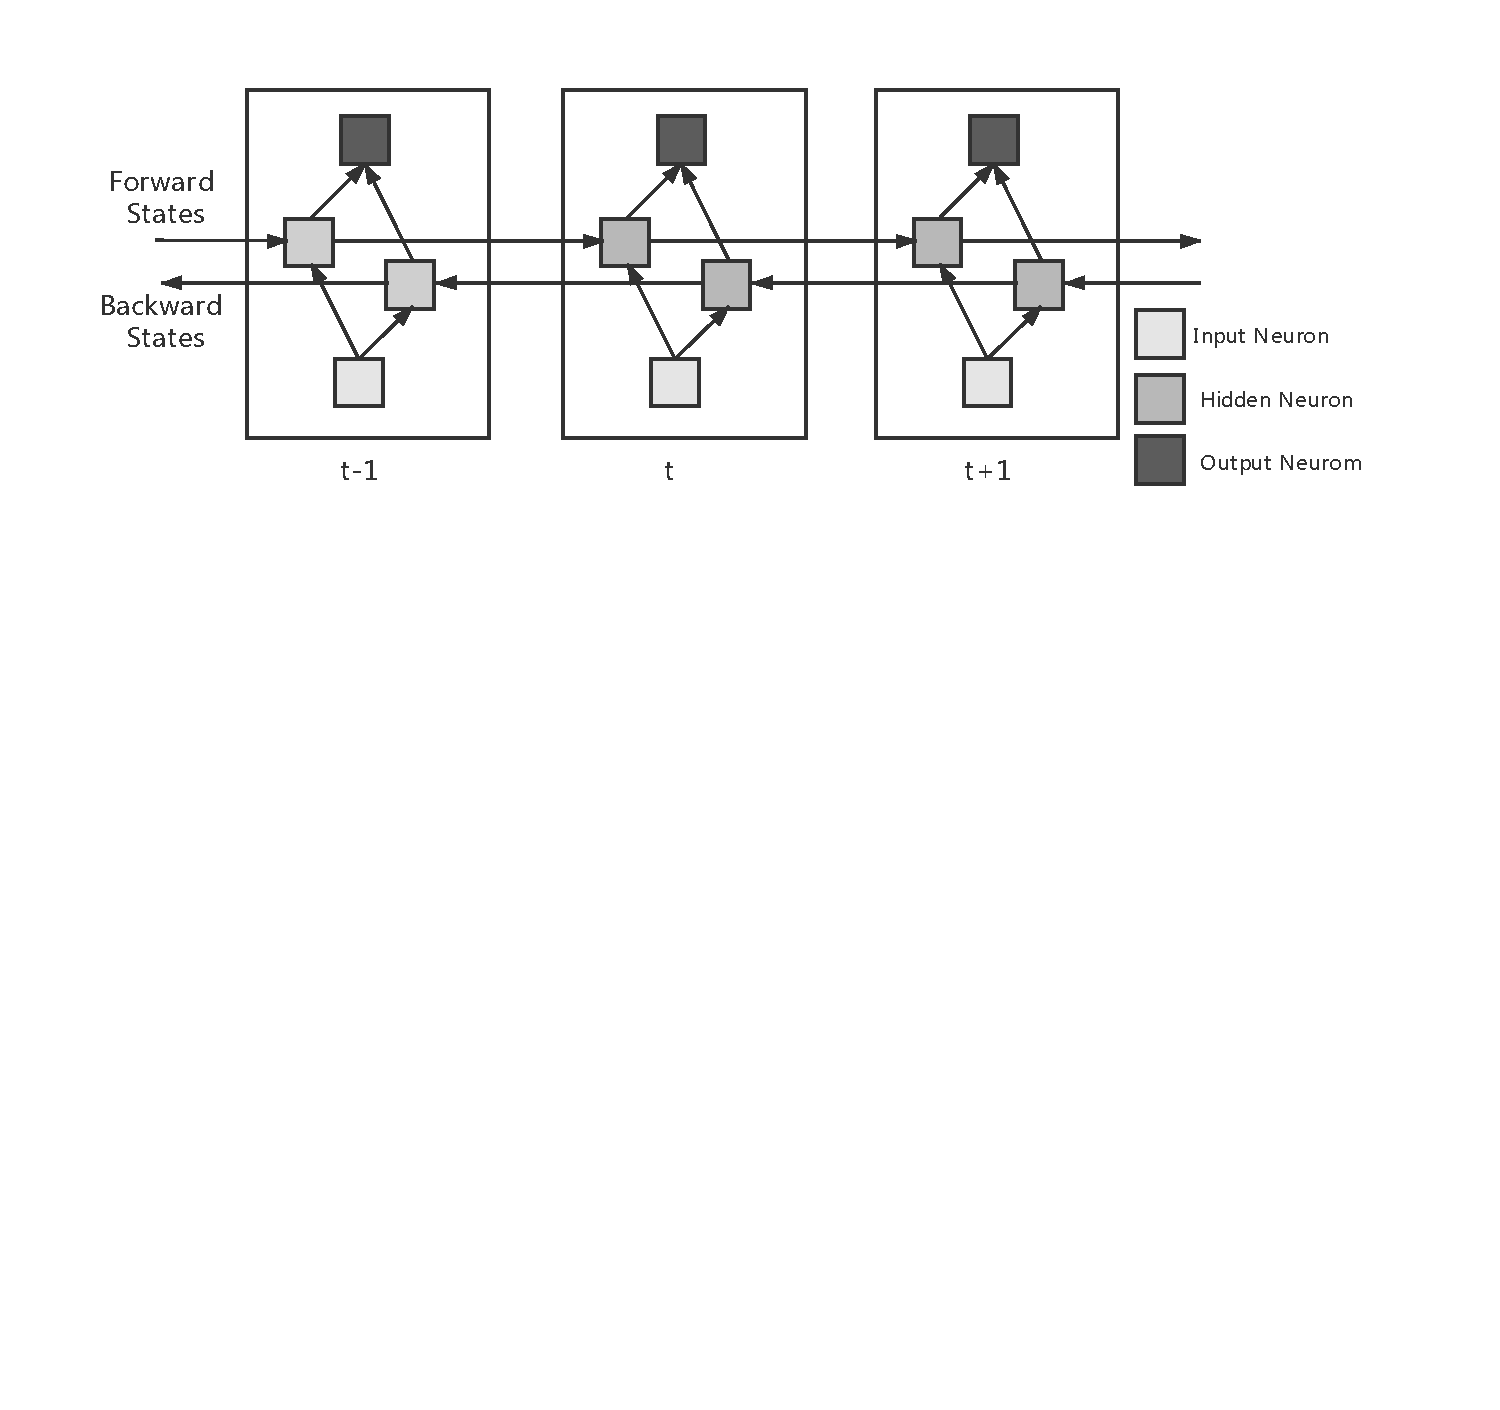
\includegraphics[width=\linewidth]{figures/BRNN.pdf}}
      \caption{The structure of Bi-RNN, the forward states are not connected to the backward state}
      \label{fig:BRNN}
    \end{figure}


    \section{Model Architecture} \label{sec:Arch}
      The architecture of the model is shown in Fig.~\ref{fig:arch}, the whole model consists of a 2D CNN sub-network and a Bi-LSTM sub-network which separately extracts high level features and predicts the yield. The input of the network is the preprocessed data which has the same planting duration of 186 days, the output of the CNN network is fed to the Bi-LSTM network which consists of 3 stacked Bi-LSTM layers followed by a fully-connect layer to give the prediction.

      \begin{figure*}[tb]
        \centering
        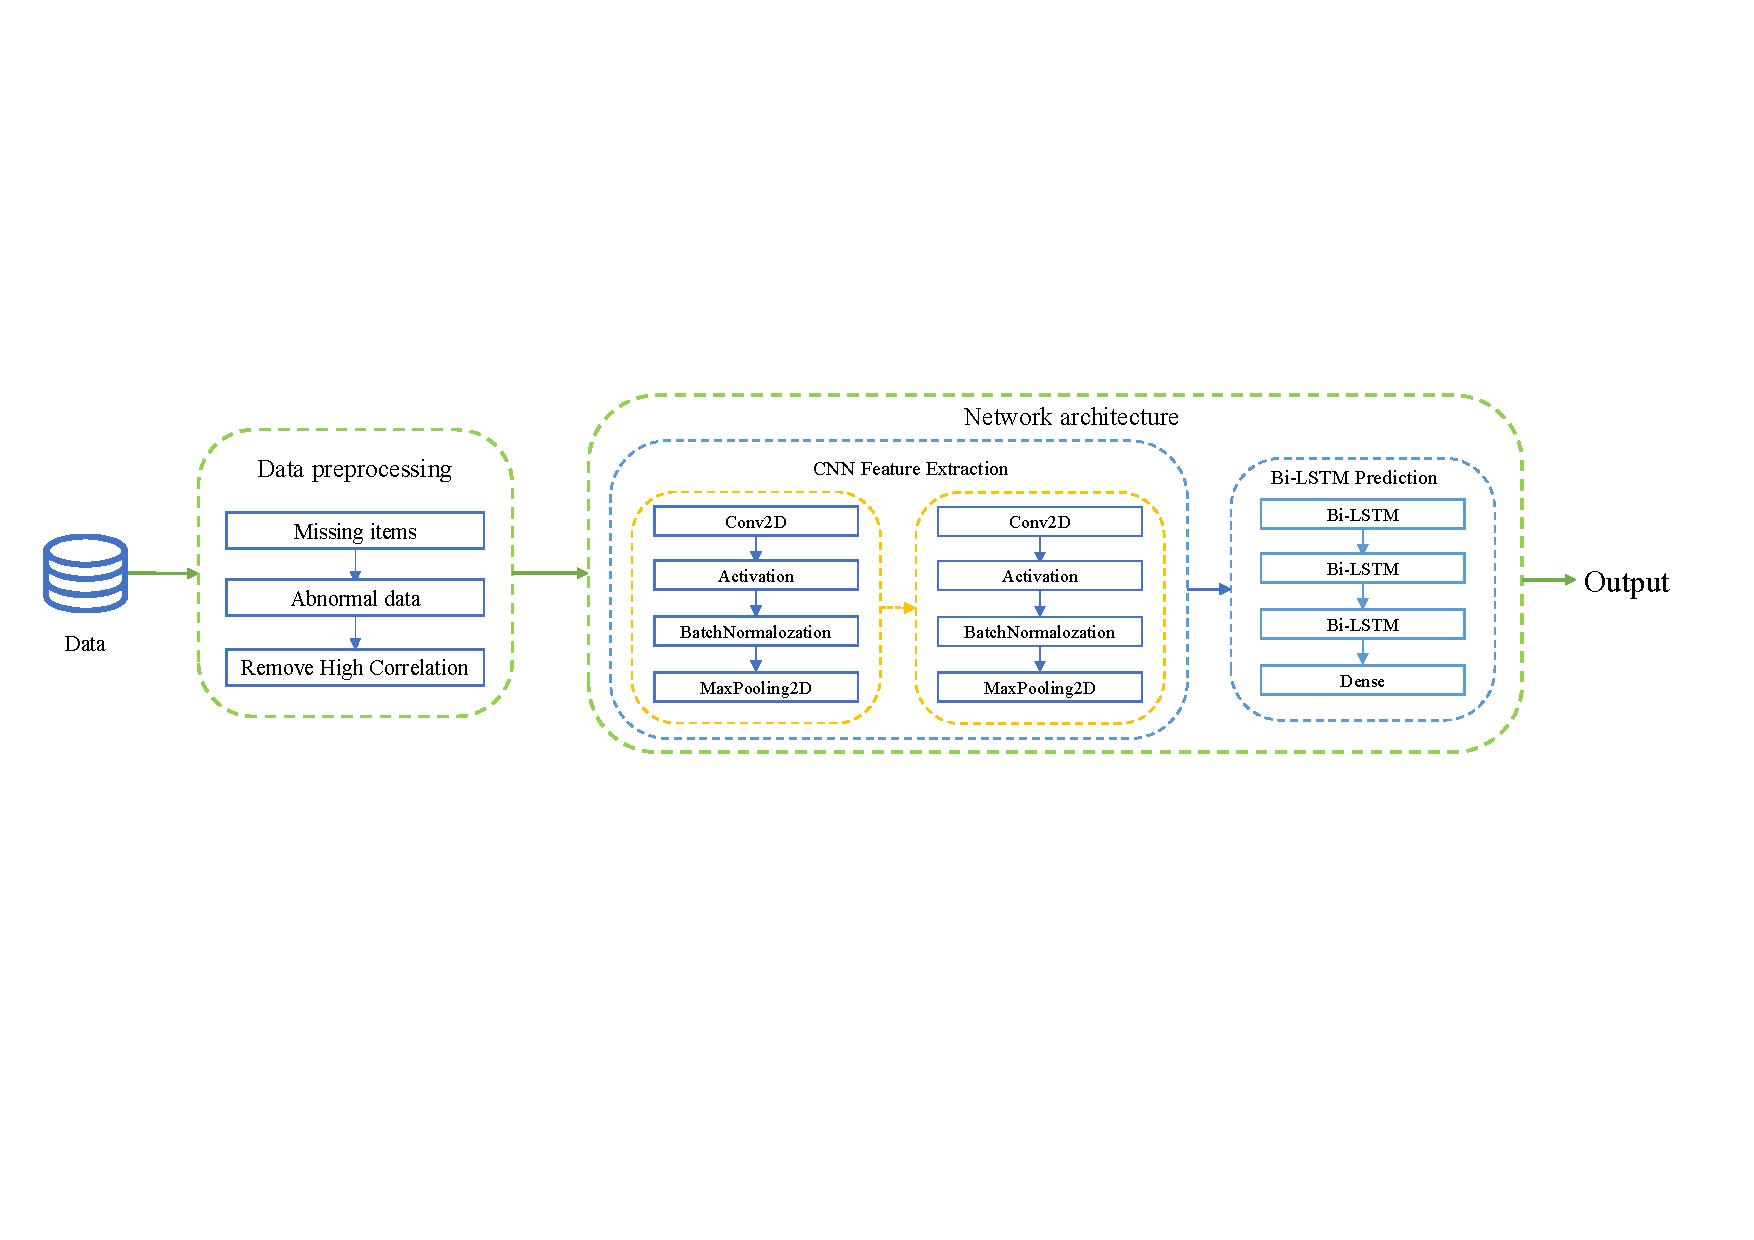
\includegraphics[width=\linewidth]{figures/new_arch.pdf}
        \caption{The architecture of the model are splited into two sub-networks, one is the CNN sub-network for feature extraction and the other is Bi-LSTM sub-network for yield prediction.}
        \label{fig:arch}
      \end{figure*}

      The CNN network is employed for feature extraction, there are two same Conv2D structure stacked in the CNN sub-network which contains a Conv2D layer, Relu activation layer, BatchNormalization layer and Maxpooling layer. The kernel size of the Conv2D layers is $1\times2$, and the first one has 32 filters while the second one has 64 counterparts. The Conv2D layers are in the timedistributed wrapper which makes the Conv2D layer do the same calculation on every time pieces. Then, Conv2D layers are first followed by a activation layer with the activation function ReLU (Rectified Linear Units) (\ref{eq:relu}) and then followed by a batch normalization layer and a max-pooling layer whose kernel size is $1\times2$. And at the end of the CNN sub-net, the output is reshaped to $184\times64$ by a reshape layer to fit the input shape request of Bi-LSTM sub-network. Batch normalization regularize the CNN to mitigate the overfitting and the pooling layers improve network's generalization, robustness to small distortions and reduces dimensionality.

      \begin{equation}
        ReLU=\max(0, x)
        \label{eq:relu}
      \end{equation}
      
      There are three stacked Bi-LSTM layers followed by two dense layer to predict the yield in Bi-LSTM sub-network. By the Bidirectional wrapper, the three LSTM layers can utilize the information from both positive time direction and negative time direction. ALl of three layers have 64 filters and both of the kernel regularizer and the recurrent regularizer are set to be the L2 with the property of 0.0001. The weight initializer we choose the Glorot normal initializer, also called Xavier normal initializer, proposed by Glorot in 2010\cite{glorotUnderstandingDifficultyTraining2010}. It initialize the weights by drawing samples from a uniform distribution within $[-B, B]$, where $B$ can be calculated by (\ref{eq:Glorot}), in which the $F_{i}$ represents the number of input units in the weight tensor and $F_o$ represents the number of output units. The three stacked Bi-LSTM structure are followed by two dense layer, the first one has 32 units and the second one has 1 units, both employ the l2 kernel regularization and are initialized by the Glorot normal initializer.
      
      \begin{equation}
        B = \sqrt{\frac{6}{F_{i} + F_{o}}}
        \label{eq:Glorot}
      \end{equation}

      In the procedure of training, the accuracy on the training dataset might improve, but the performance begins to reduce at a certain point on the data not yet seen by the model. To make sure the real-world performance of the model, earlystopping callback function was employed, such function was set to monitor the cross validation MSE. The train will end when that value has stopped improving after 10 epochs consecutively. The total epoch with batch size of 16 was set to be 1000 under the regulation of earlystopping callback, and the gradient descent on top of the adaptive momentum (ADAM) optimizer was choose.

\section{Experiment} \label{sec:ex}
  \subsection{Data Preprocessing} 
    The dataset includes data of winter wheat yield in the U.S with local climate conditions in 2013 and 2014, and contains 150 counties from 5 states and has 26 features, 360042 entries in total.

  \subsubsection{Missing items}
    There are 654 missing items in the dataset, accounting for 1.81\% of the total data volume. Deleting an entry with missing items may result in the decline of continuity of data in a certain location due to the characteristics of crop growth that disaster of someday will cause a great reduction of output. Filling the missing items with the nearest and most recent entry due to the continuity of climate data in both space and time. For a isolated miss item, it is filled by its spatial and temporal adjacent items, and for continuous time missing items, they will be filled from both ends to the middle one.

  \subsubsection{Abnormal data}
    By going through the data, an apparent anomaly was found in the yield which is shown in Fig.~\ref{fig:drop-data}(a). There are entries having nonzero yield with a relatively short period of time from being seeded to harvest which was recorded by column \textit{DayInSeason}. To ensure a uniformed input shape and drop such abnormal data, we dropped data from locations who have recorded for less than 186 days. After doing so, there are 901 locations left in the dataset which all have the same planting duration of 186 days.

  \begin{figure} 
      \centering
      % TODO: 重绘图a
    \subfloat{%
        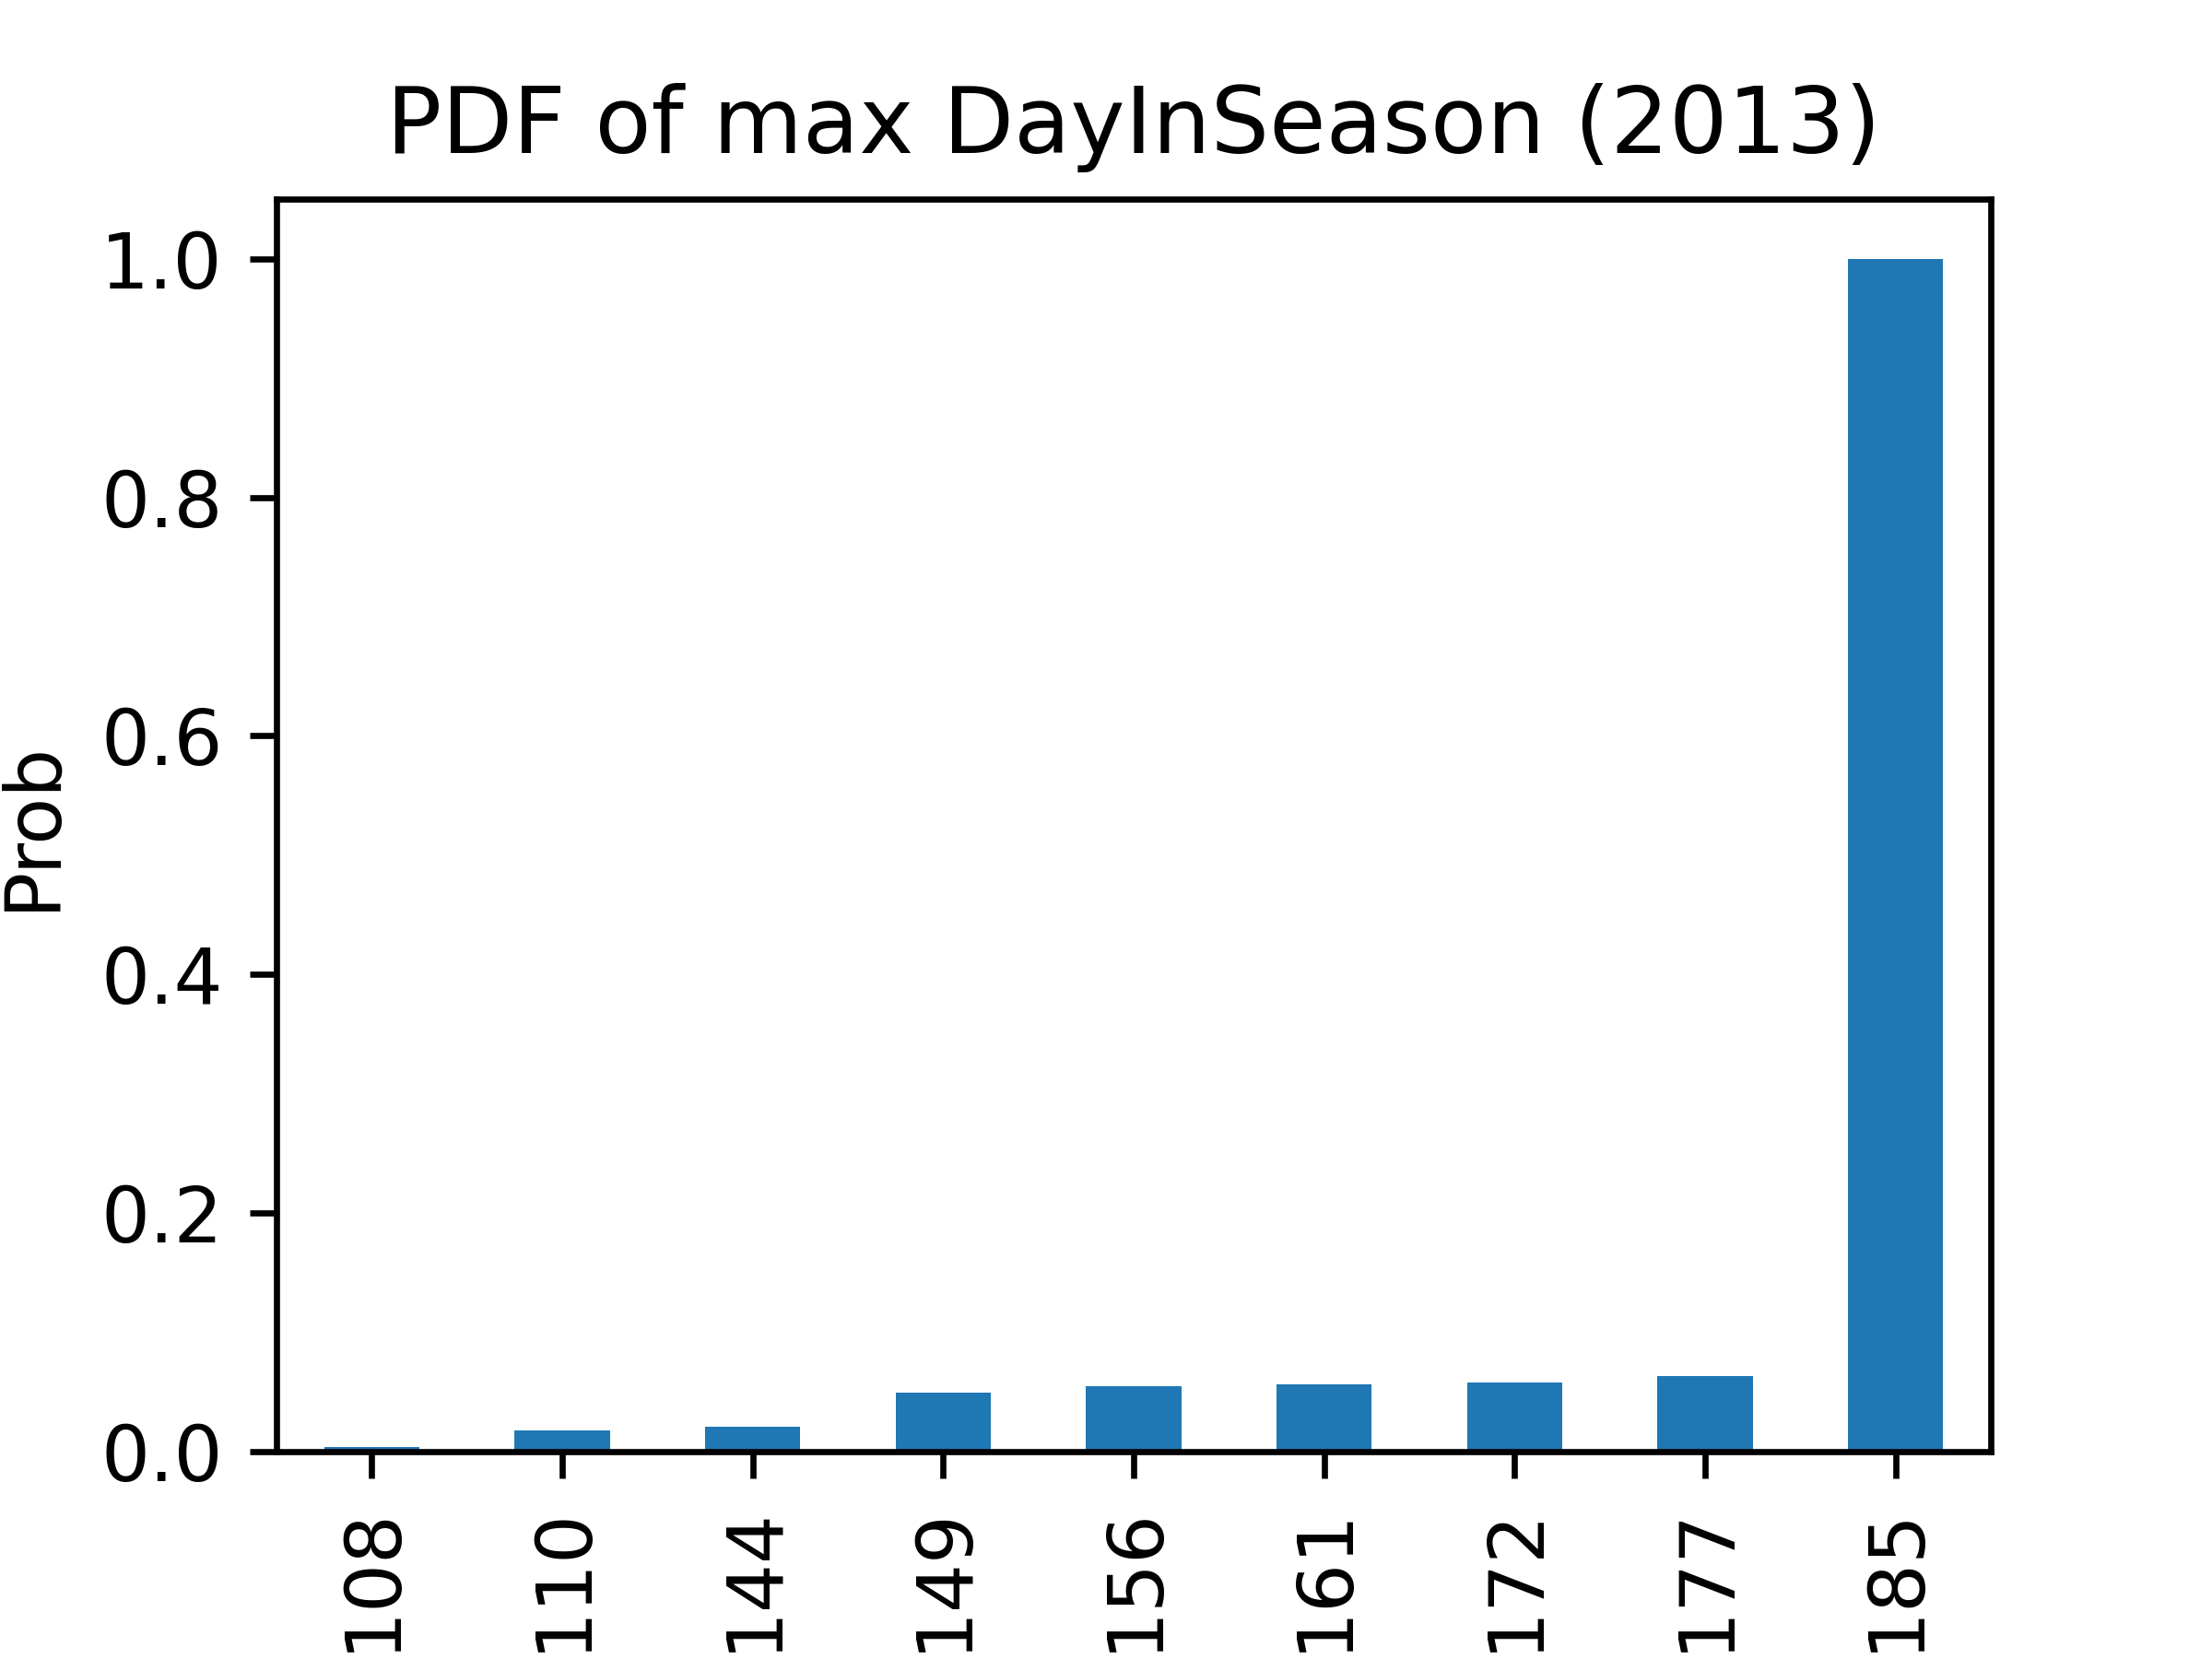
\includegraphics[width=0.45\linewidth]{./figures/PDF of max DayInSeason (2013).png}}
      \hfill
    % \subfloat[\label{1b}]{%
          % 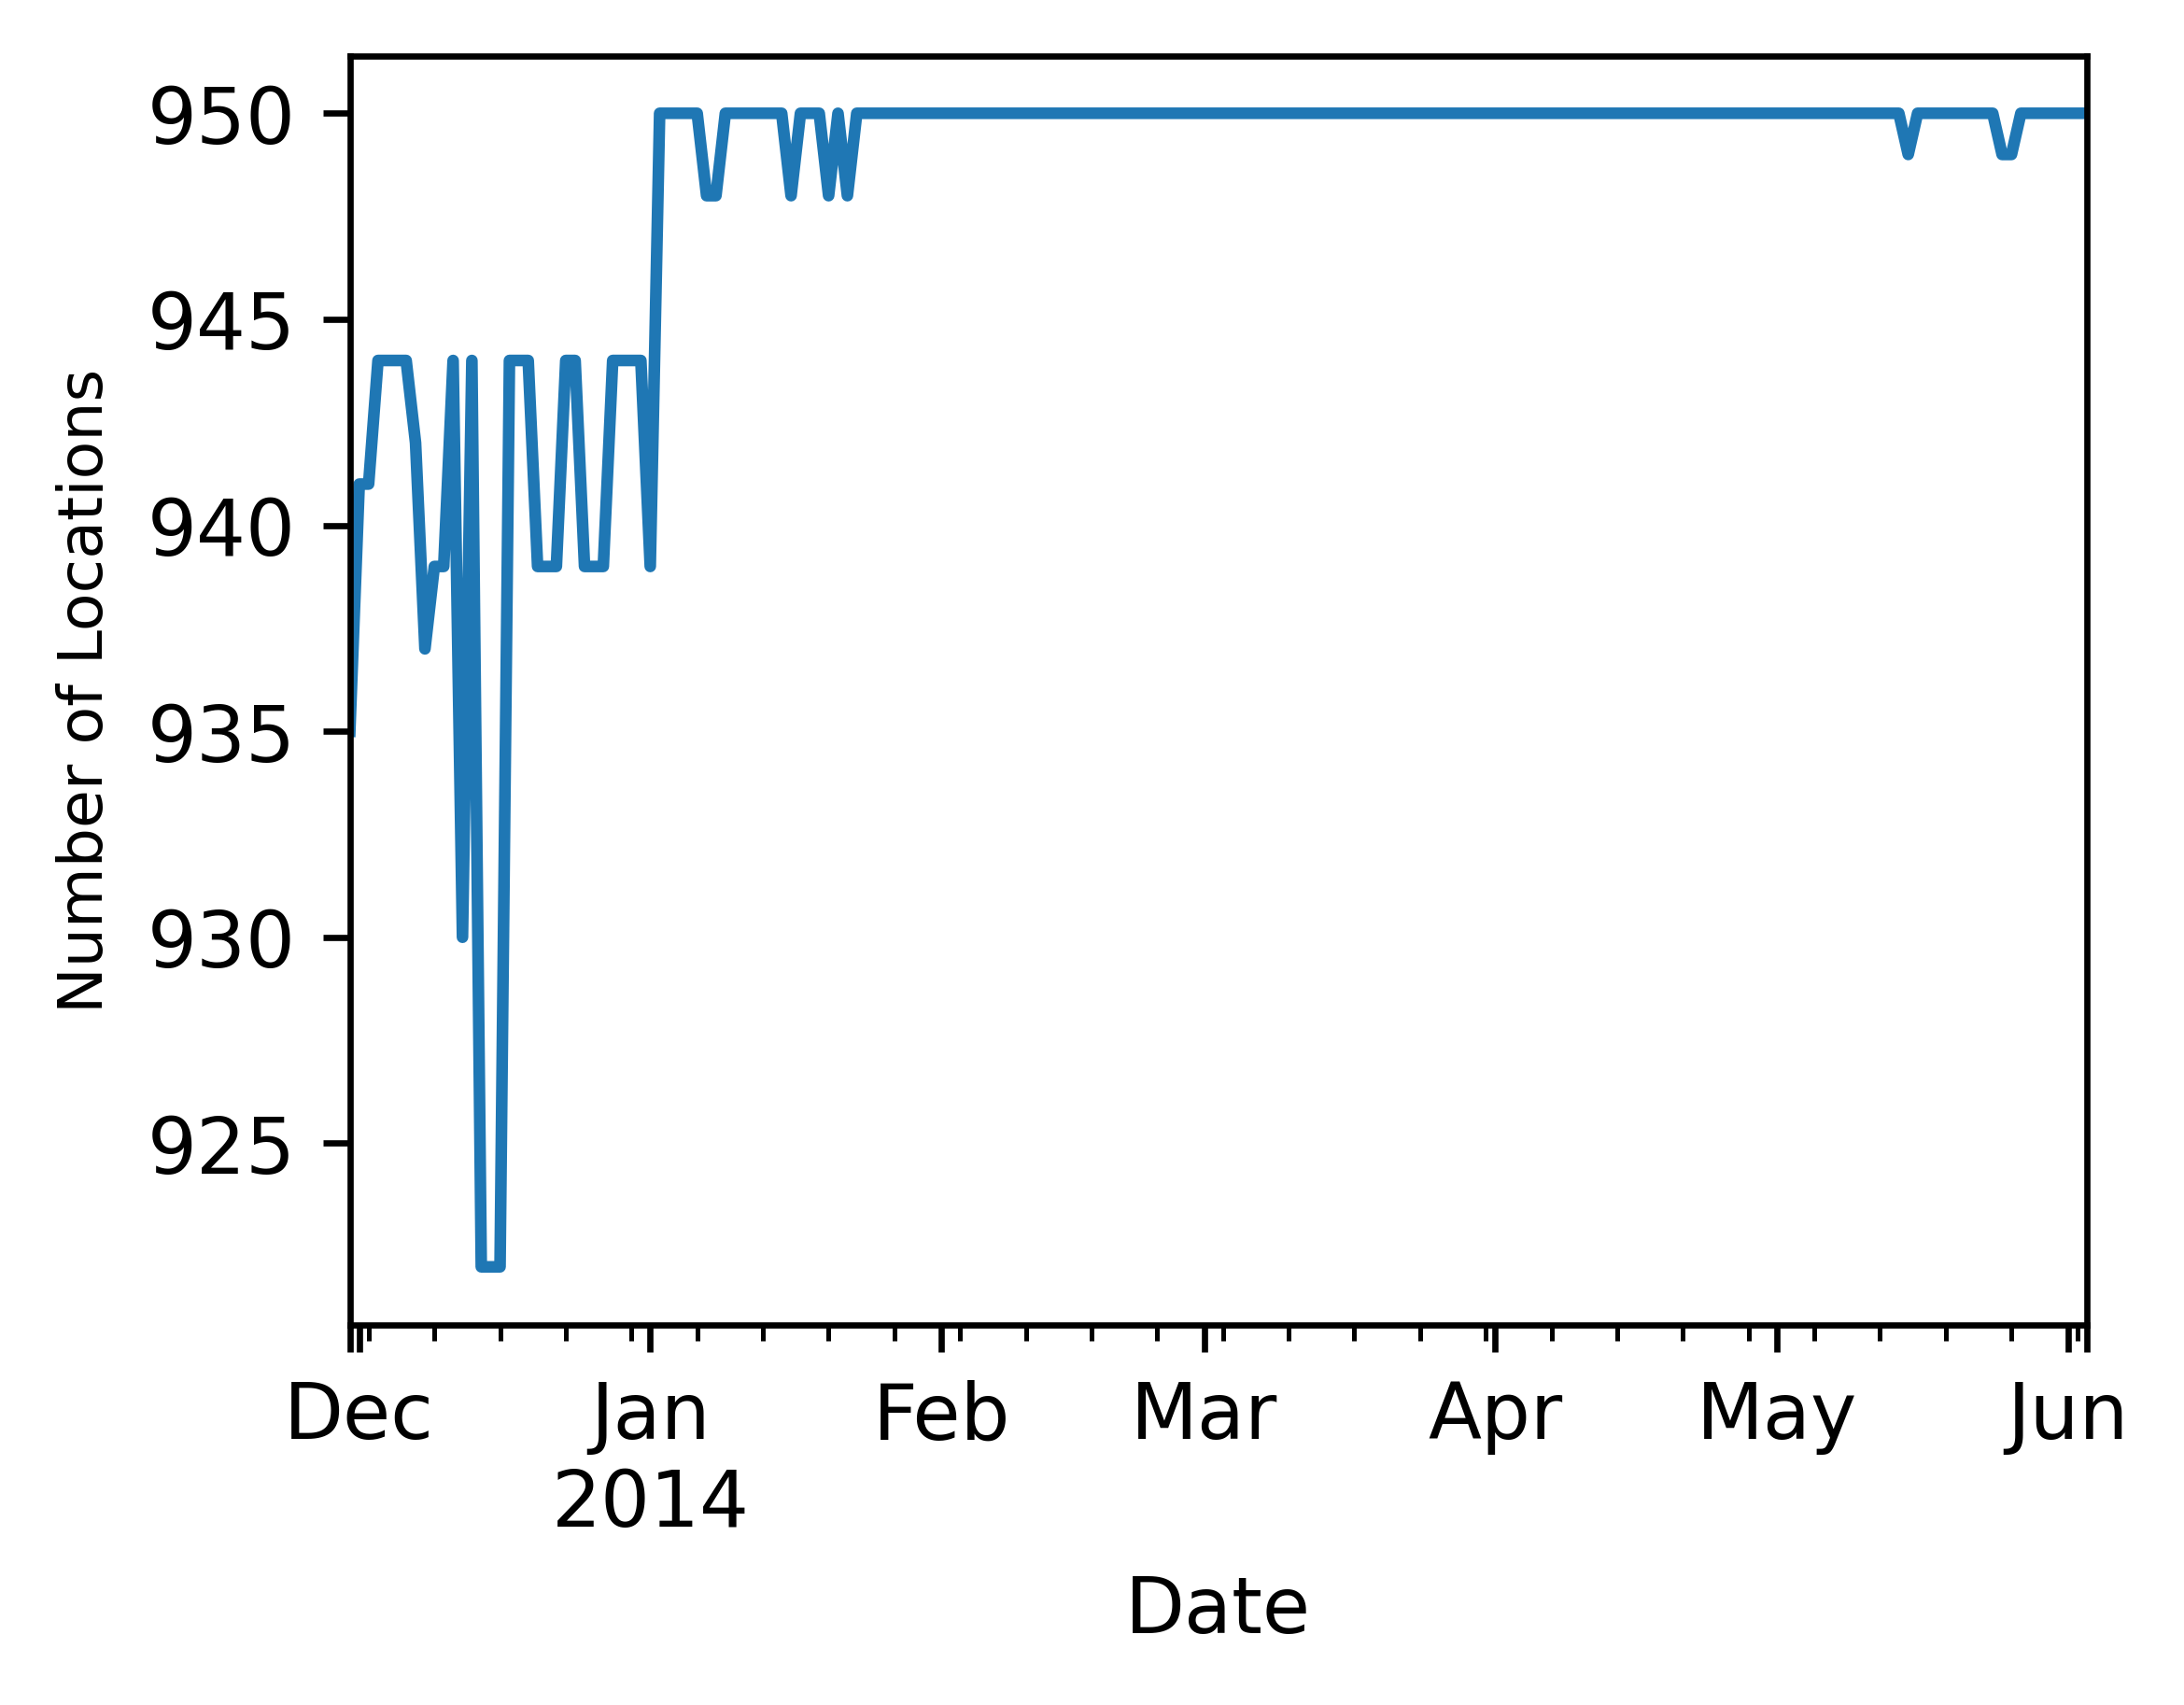
\includegraphics[width=0.45\linewidth]{./figures/date&locations(origin).png}}
      % \\
    % \subfloat[\label{1c}]{%
          % 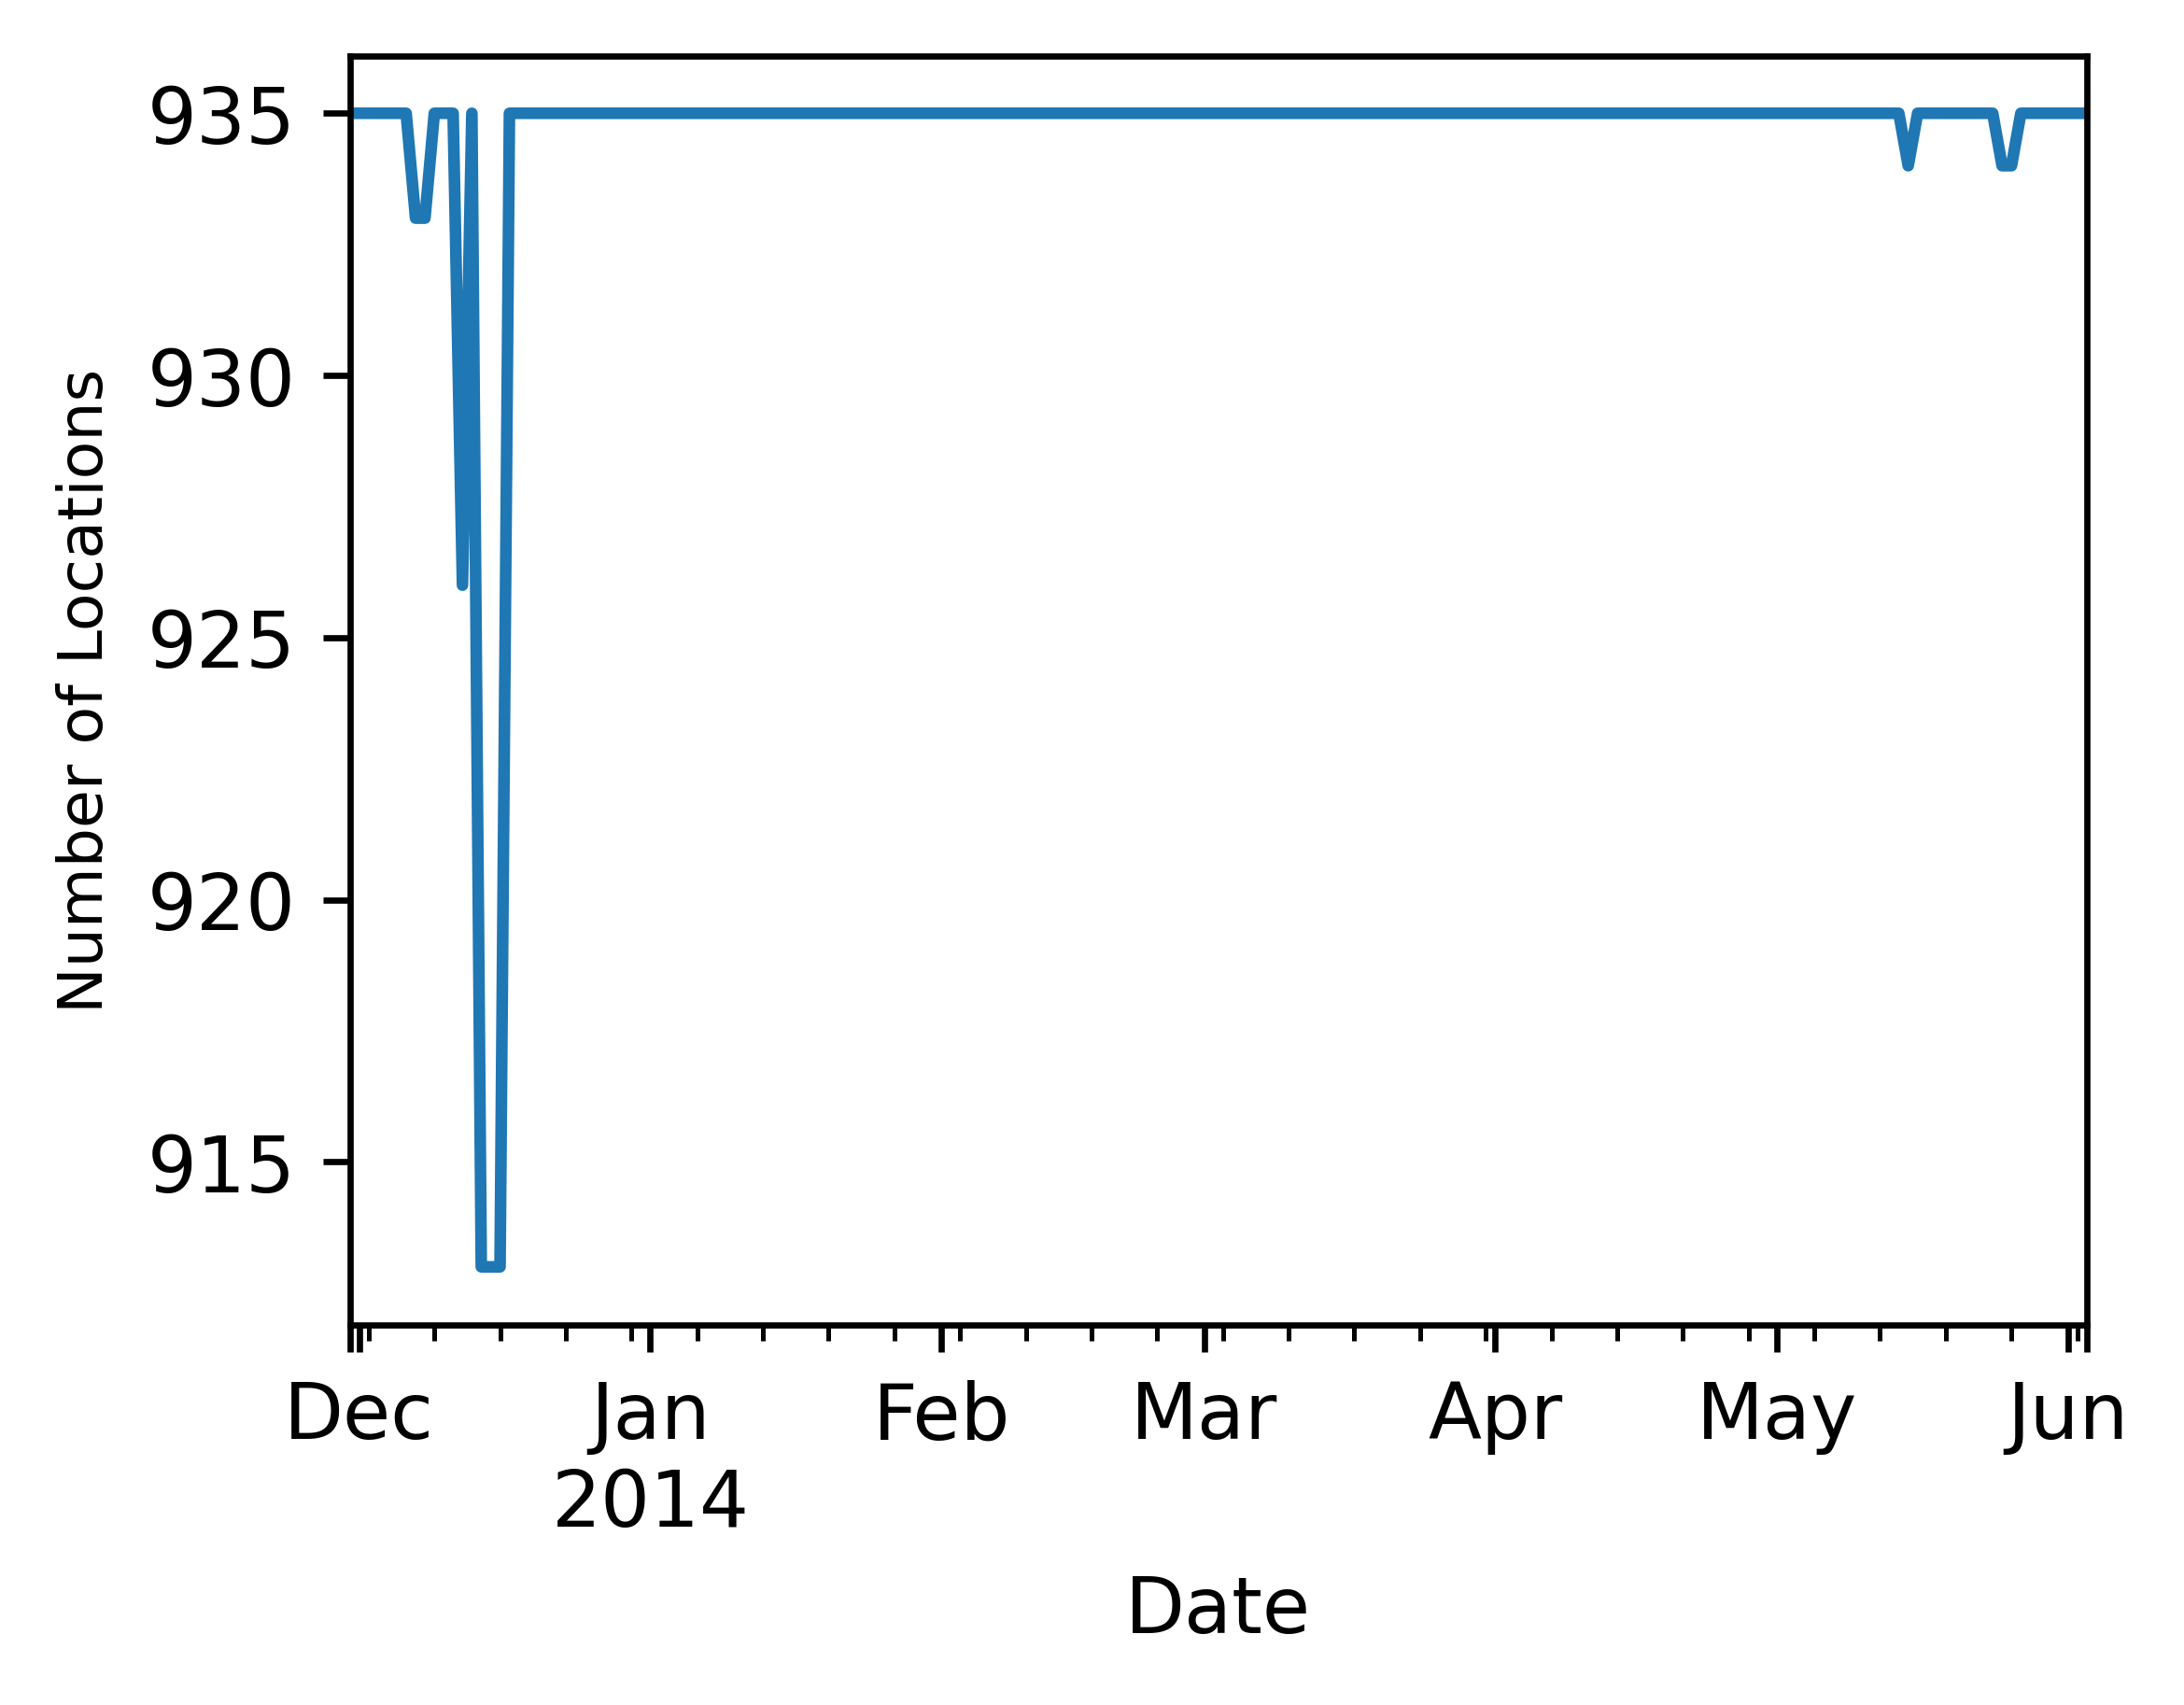
\includegraphics[width=0.45\linewidth]{./figures/date&locations.png}}
      % \hfill
    \subfloat{%
          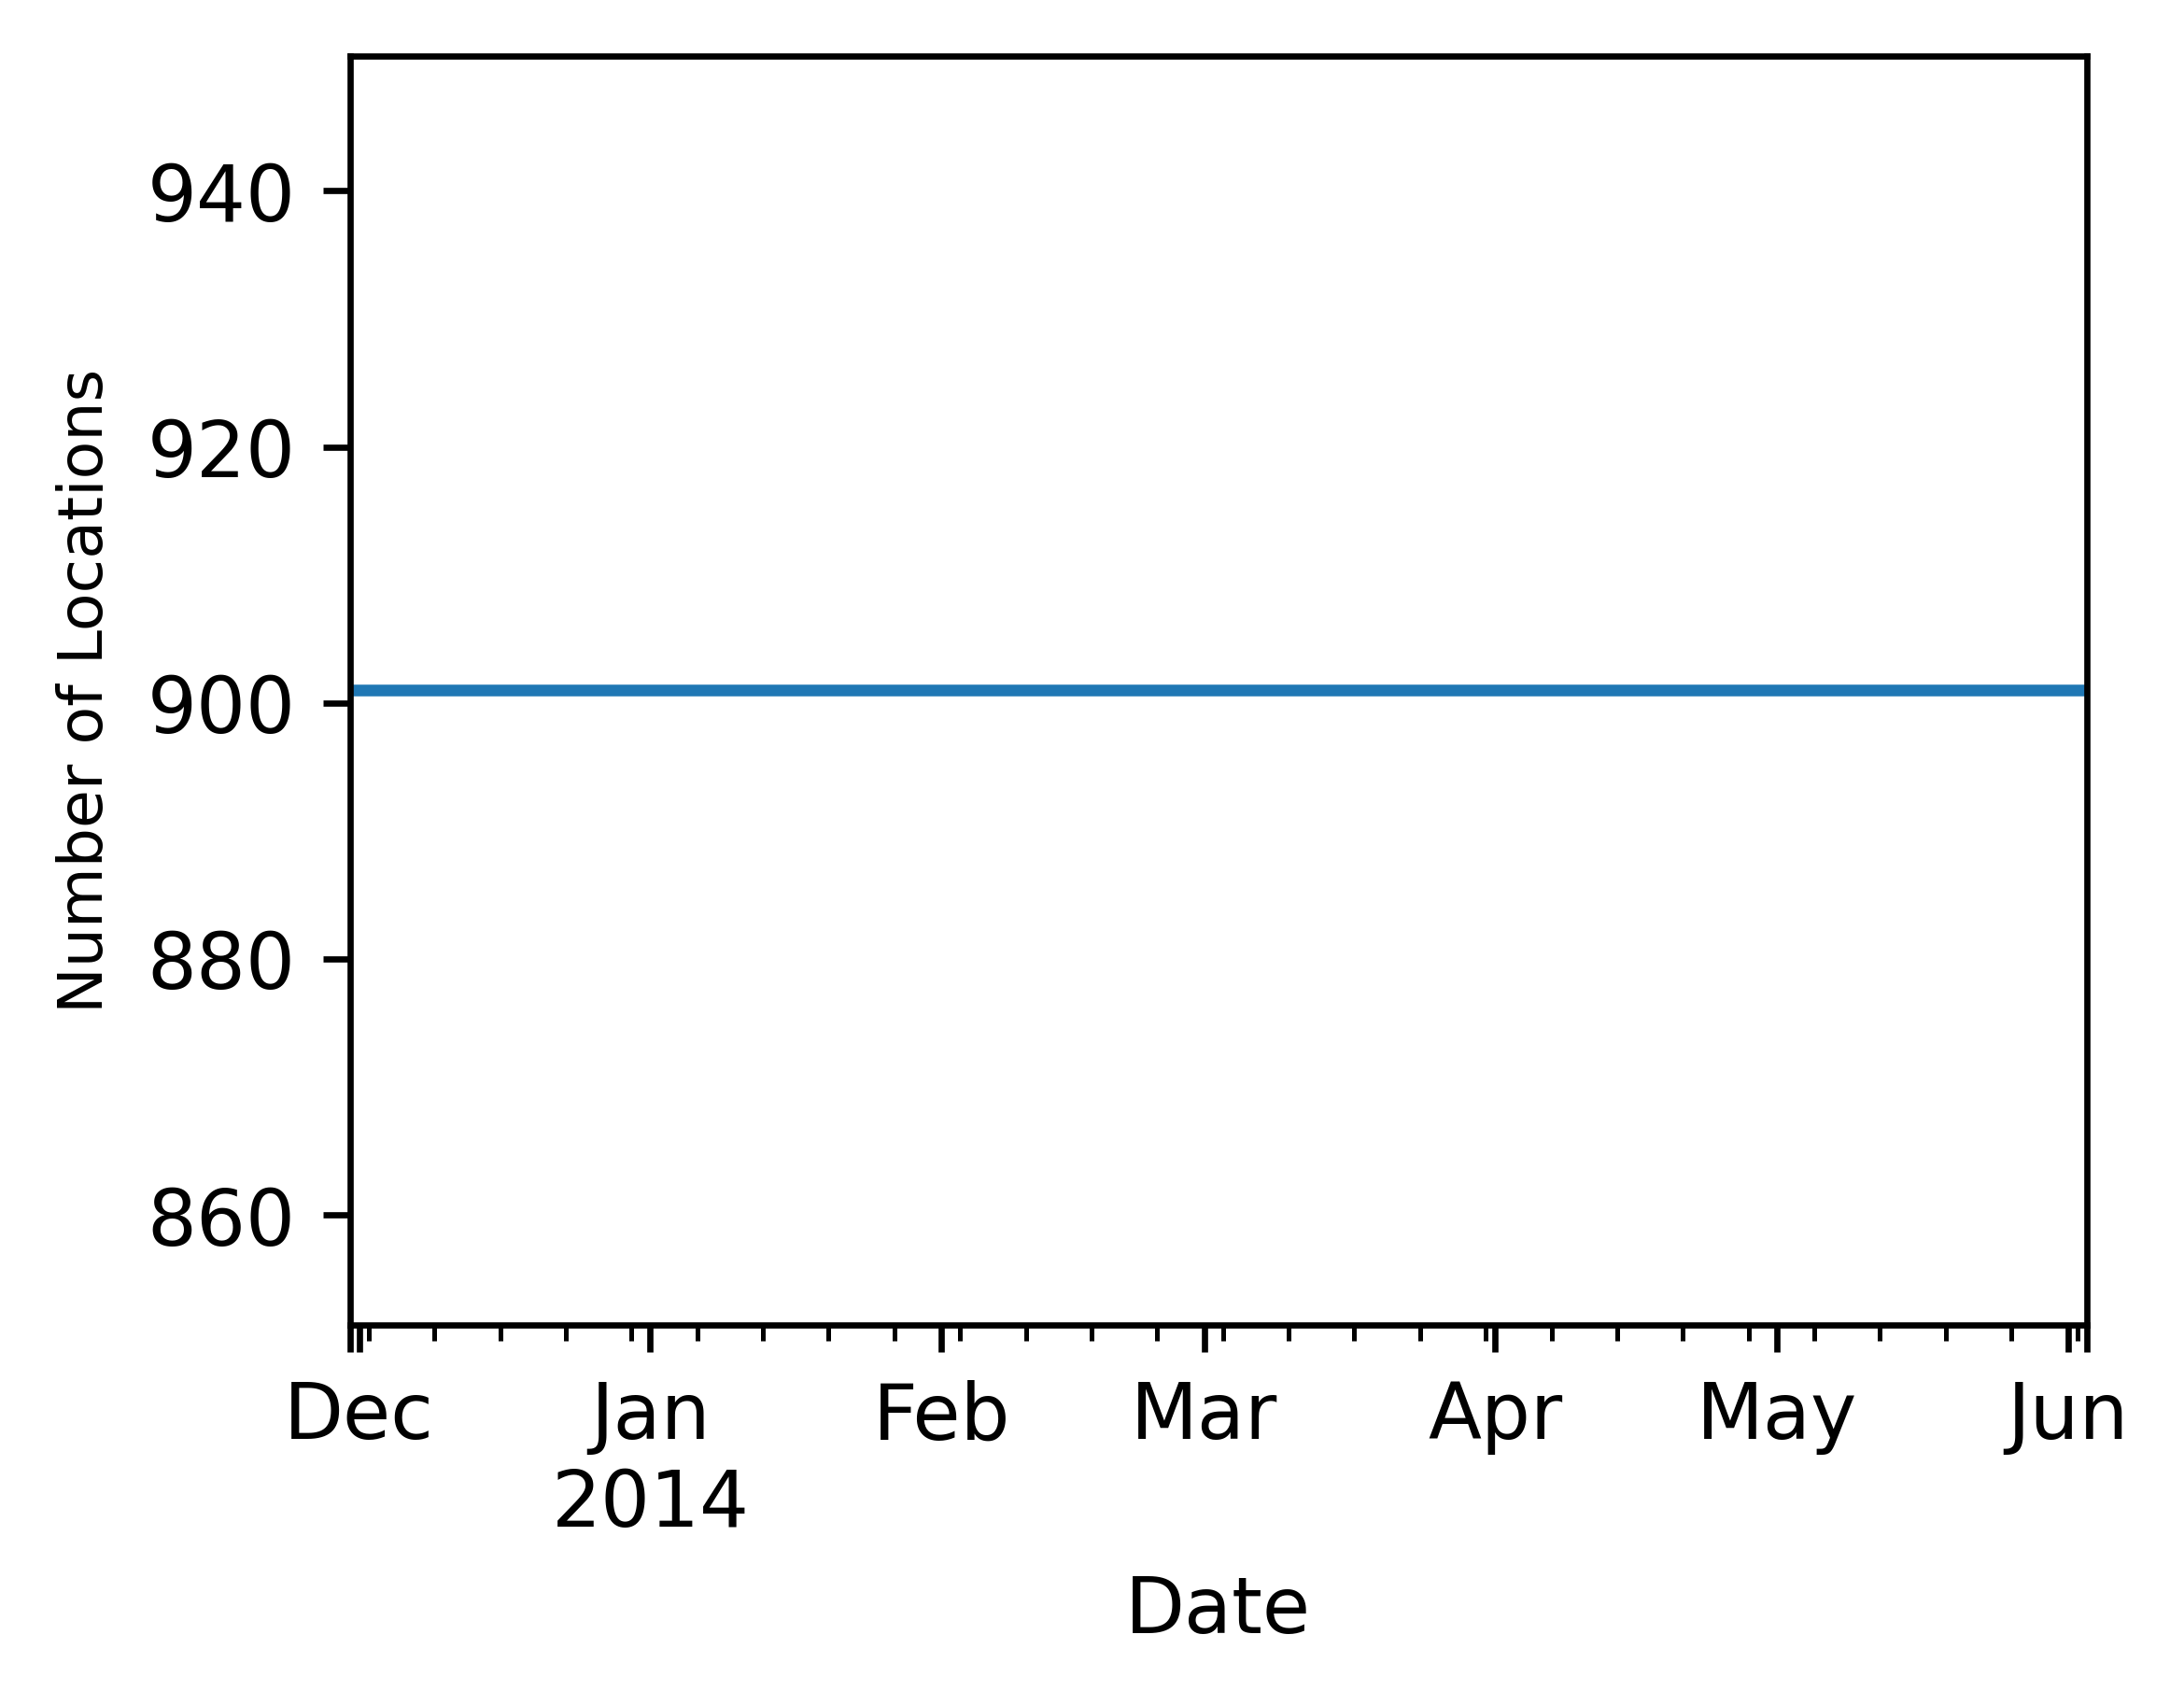
\includegraphics[width=0.45\linewidth]{./figures/date&locations(clean).png}}
    \caption{(a) shows the location  }
    \label{fig:drop-data}
  \end{figure}

  \subsubsection{Map visualization}
  For data with location, map visualization can always help us find some intuitive relations between location and target. According to Fig.~\ref{fig:Map_visual}-(b), there are two intuitive conclusions:
  \begin{itemize}
      \item The yield in the northern growing areas was significantly higher than that in the south. 
      \item In the south growing areas, the more east the locations are the high the yields are.
  \end{itemize}

  \begin{figure*}[htb]
      \centering
    \subfloat{%
        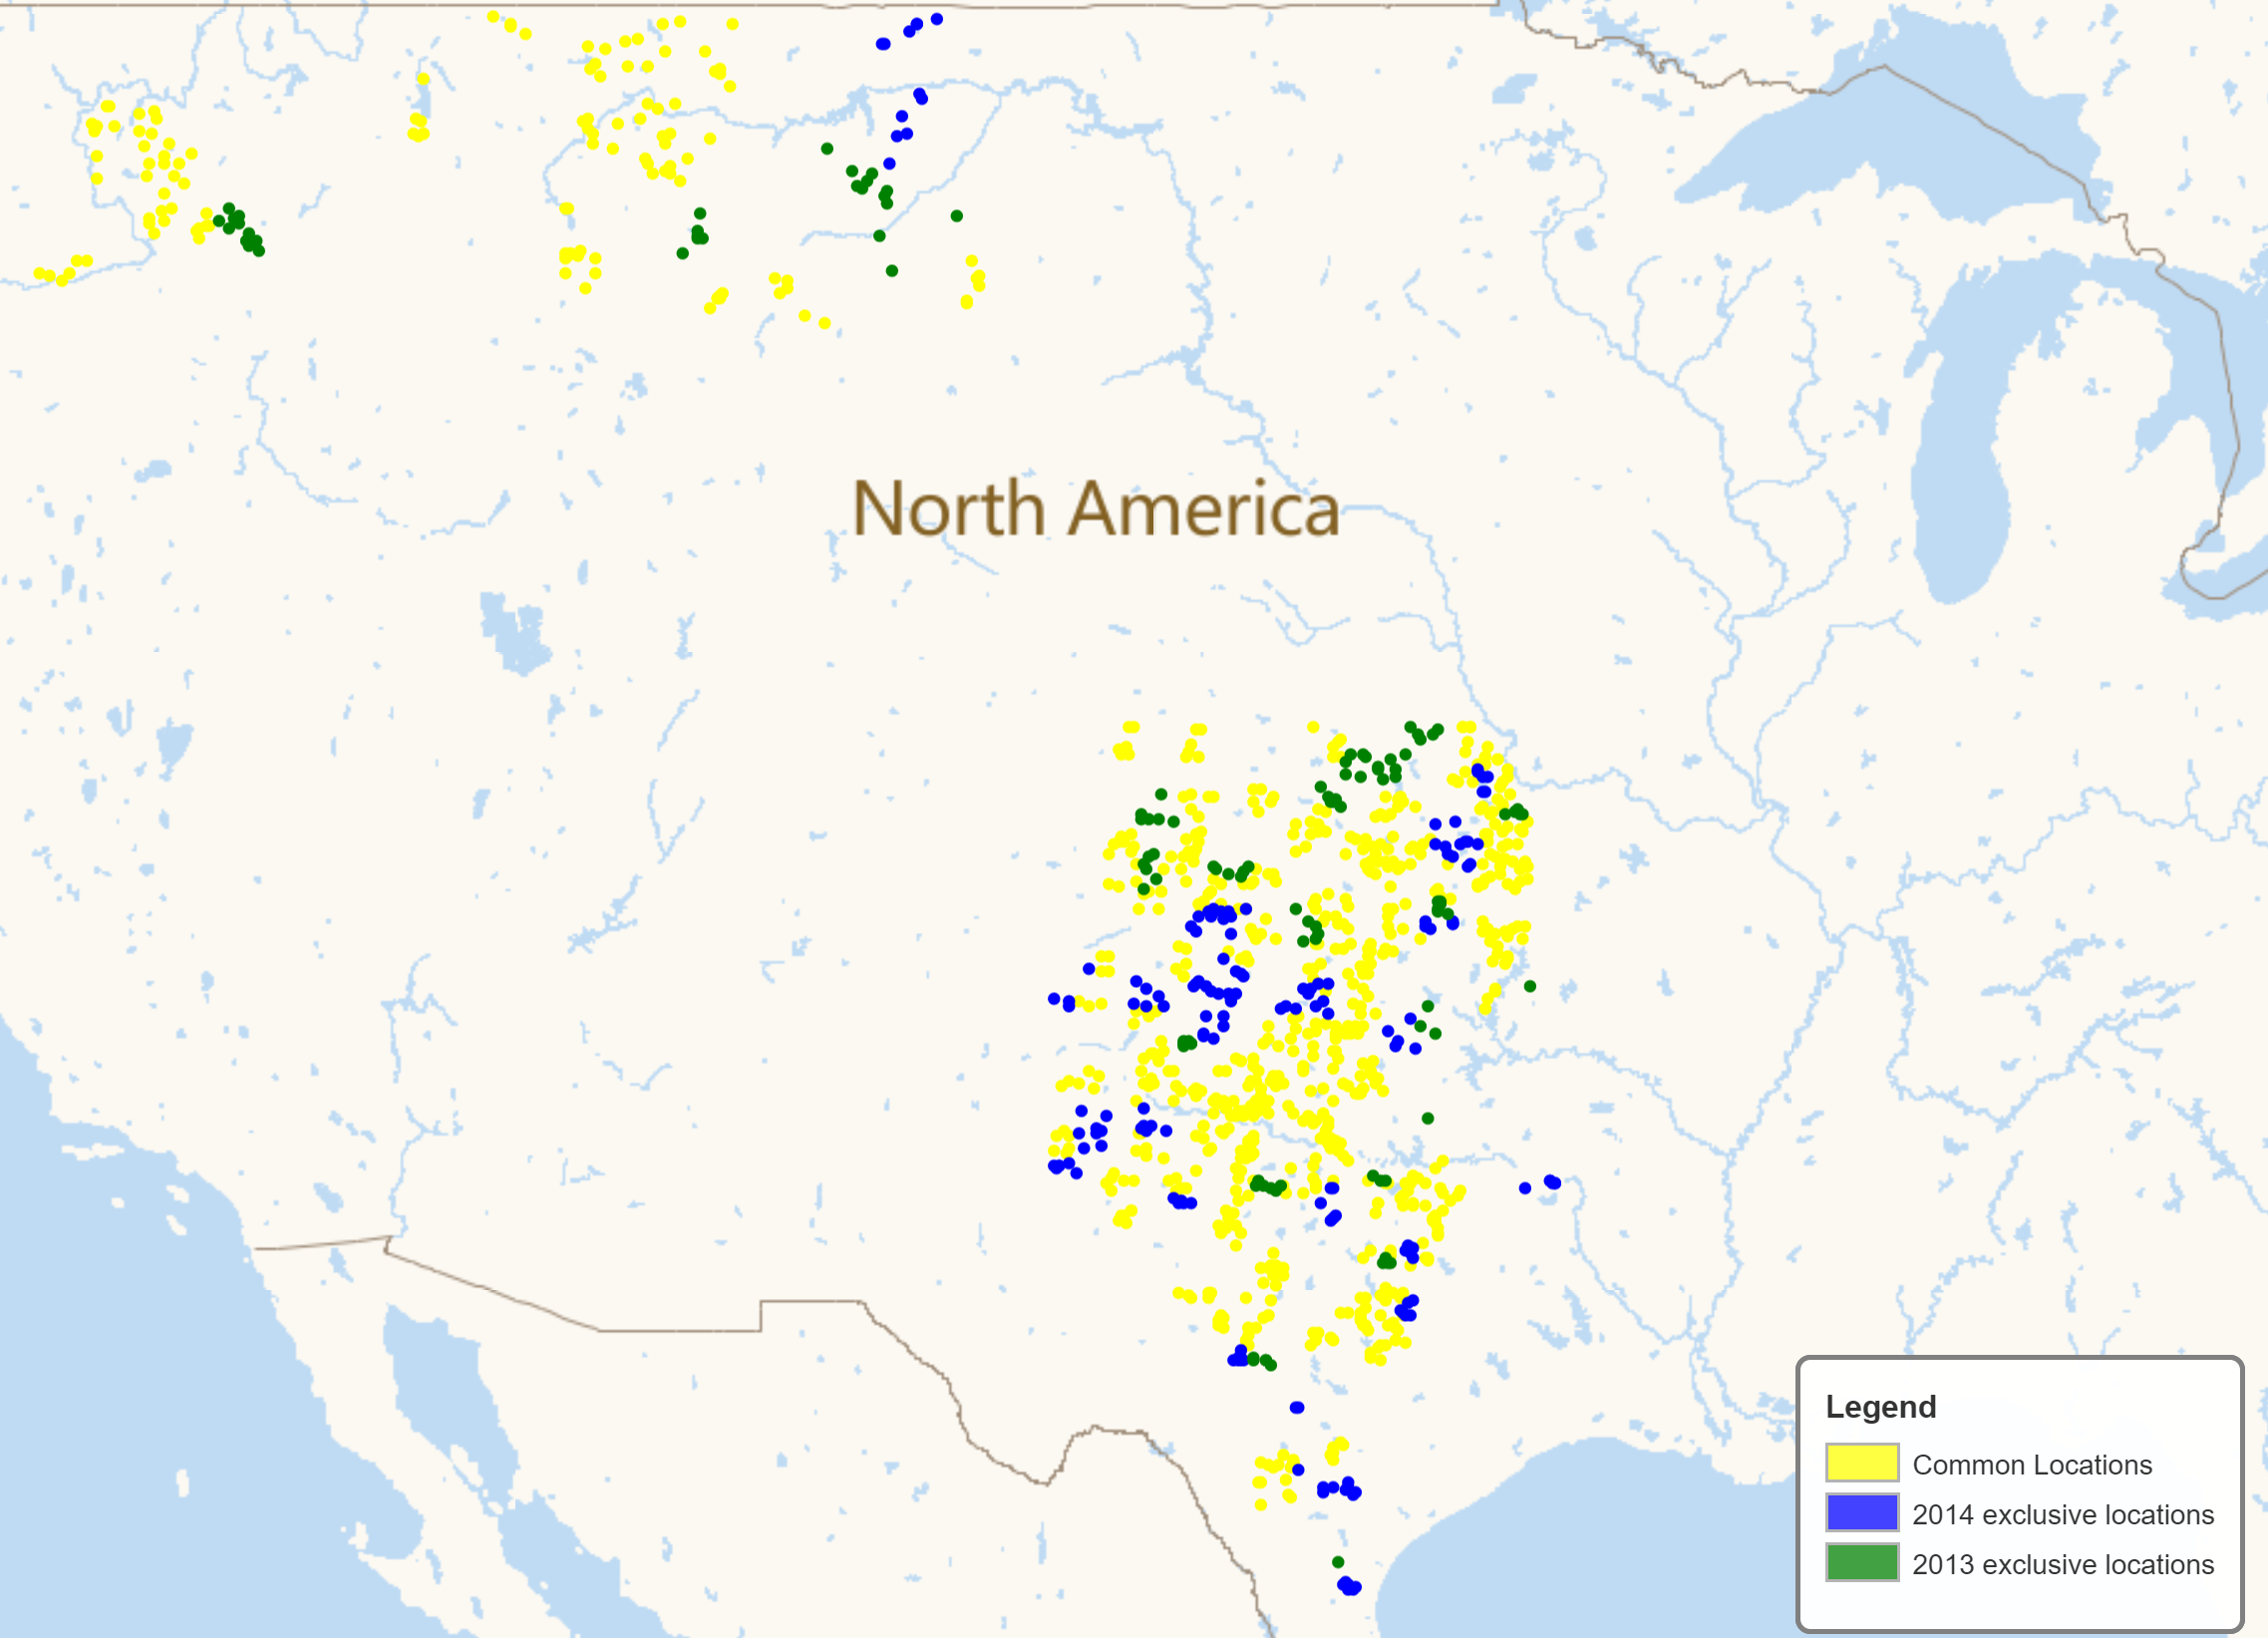
\includegraphics[width=0.45\linewidth]{./figures/data_locations.png}}
      \hfill
    \subfloat{
          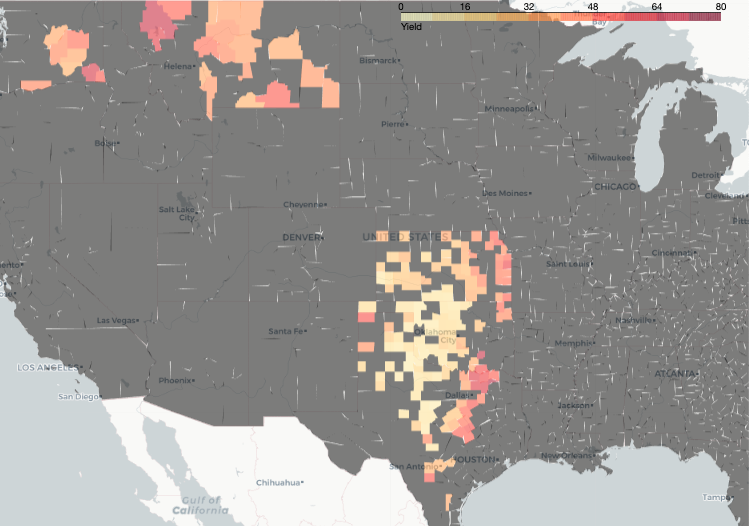
\includegraphics[width=0.45\linewidth]{./figures/map.png}} 
    \caption{(a)shows the location of all data being collected, yellow points represent locations monitored for two years which accounts for most of the locations (b)shows the yield varying by locations}
    \label{fig:Map_visual}
  \end{figure*}

  \subsubsection{Cut high correlation features}
    There is significant multicollinearity between some features in the dataset, that multicollinearity can lead to errors and distortions in results\cite{farrarMulticollinearityRegressionAnalysis1967}. By calculating the correlation coefficient between the features, some features with abnormal high correlation which reaches 99\%. Table.~\ref{tab:correlation} shows the pairs of features whose correlation high than 90\%. Before the data is feed to the model, these columns with high correlation accompany with some yield irrelevant columns including \textit{State}, \textit{Location} e.t. are cut out from the original dataset.
    \begin{table}[htbp]
      \caption{Features correlation high than 90\%}
      \begin{center}
        \begin{tabular}{|c|c|c|c|c|}
          \hline
          Feature 1 & Feature 2 & cor1 & cor2 & cor3\\
          \hline
          apparentTempMin & TempMin     & 0.99 & -0.04 & -0.06 \\
          apparentTempMax & TempMax     & 0.99 & -0.14 & -0.15 \\
          precipIntensity & precipIntensityMax & 0.91 & 0.04  & 0.03  \\
          dewPoint & tempMin & 0.91 & 0.01  & -0.06 \\
          apparentTempMin & dewPoint & 0.90 & -0.04 & 0.01 \\
          \hline
          \multicolumn{5}{l}{$^{\mathrm{a}}$cor1: correlation between feature1 and feature2} \\
          \multicolumn{5}{l}{$^{\mathrm{b}}$cor2: correlation between feature1 and yield} \\ 
          \multicolumn{5}{l}{$^{\mathrm{c}}$cor3: correlation between feature2 and yield} \\
        \end{tabular}
        \label{tab:correlation}
      \end{center}
    \end{table}

  \subsection{Algorithm Evaluation}
    Before testing, use the \textit{Min-Max} method (\ref{eq:standarlize}) to standardize the data, then the data was fed to the model.

    \begin{equation}
    x_i := \frac{x_i-\min \left( x_i \right)}{\max \left( x_i \right) -\min \left( x_i \right)}
    \label{eq:standarlize}
    \end{equation}

    To evaluate the performance of the algorithms, a certain part (20\%) of data was randomly set apart as validation set. Such setting can make the algorithms have the same baseline to compare to each other. We use both mean-square-error (MSE) and the coefficient of determination denoted as $R^2$ to estimate the performance of the algorithms. The $R^2$ score can be calculated by (\ref{eq:tot})-(\ref{eq:r2}).

    \begin{equation}
      SS_{tot} = \sum_{i}(y_i-\bar{y})^2
      \label{eq:tot}
    \end{equation}

    \begin{equation}
      SS_{res} = \sum_{i}(y_i-f_i)^2=\sum_ie_i^2
      \label{eq:res}
    \end{equation}

    \begin{equation}
      R^2 = 1-\frac{SS_{res}}{SS_{tot}}
      \label{eq:r2}
    \end{equation}

\subsection{Result}
  Besides the Bi-LSTM model, we also tested commonly used ML algorithms and naive LSTM models, each algorithms are fed the same data except SVR whose computing complexity is too high to fed all the data\cite{clarkeAnalysisSupportVector2005}. But during the test procedure, the randomly forest shows a severe overfitting, extra efforts are done to solve such problem in Section.\ref{sec:ovf}. The results of the algorithms is shown in Table.~\ref{tab:result}.

    % TODO: 重新测试
  \begin{table}[htbp]
    \caption{Performance of algorithms}
    \begin{center}
    \begin{tabular}{|c|c|c|}
    \hline
    Algorithm                                    & MSE      & $R^2$\\
    \hline
    Random Forest \cite{liawClassificationRegressionRandomForest2002}                      &    47.85  & 0.71\\
    KNN \cite{petersonKnearestNeighbor2009}                                         & 60.65 & 0.43\\
    Polynomial regression & 108.48 & 0.24\\
    Linear regression   & 179.43 & 0.13\\
    SVR \cite{druckerSupportVectorRegression1997}                                     & 188.46 & 0.11\\
    SVR RBF kernel \cite{cristianiniIntroductionSupportVector2000}                         & 193.51 & 0.07\\
    SVR linear kernel \cite{cristianiniIntroductionSupportVector2000}                      & 197.06 & 0.06\\
    \hline
    Naive LSTM    & 45.38    &  0.73\\
    CNN-Bi-LSTM(Our method) & 12.37 & 0.84\\
    \hline
    \end{tabular}
    \label{tab:result}
    \end{center}
  \end{table}

  % Group the data by location and check the yield finding that the number of unique yields does not match that of locations, which means there are entries share the same yield. Look further into data, finding that the yield of a day is not the real yield of the current day, but the yield of final yield. What's more, the locations from the same county also share the same yield. That directly results in locations' neighborhoods get the same yields, and the algorithm can give the exact yield according to the yield.  

\subsection{Overfitting in Random Forest} \label{sec:ovf}
  The Random Forest have shown a severe overfitting in the test whose MSE reaches 0.0034. in this part, we try to find out what leads to this problem and solve it. Going through the contribution of the features in the prediction, we found that the location features (latitude and longitude) contribute more than 99\% in total, which means that the algorithm can give a exact "prediction" just base on where the farm is.

  We have tried three progressive methods to solve the problem. First, simply remove the longitude and latitude columns from the dataset and run the test again. Learning curve of the result shown in Fig.~\ref{fig:of}(a), the problem was not solved but tell us that it is not the location but some other factors cause the overfitting. 

  \begin{figure}[!htb]
    \centering
  \subfloat{%
      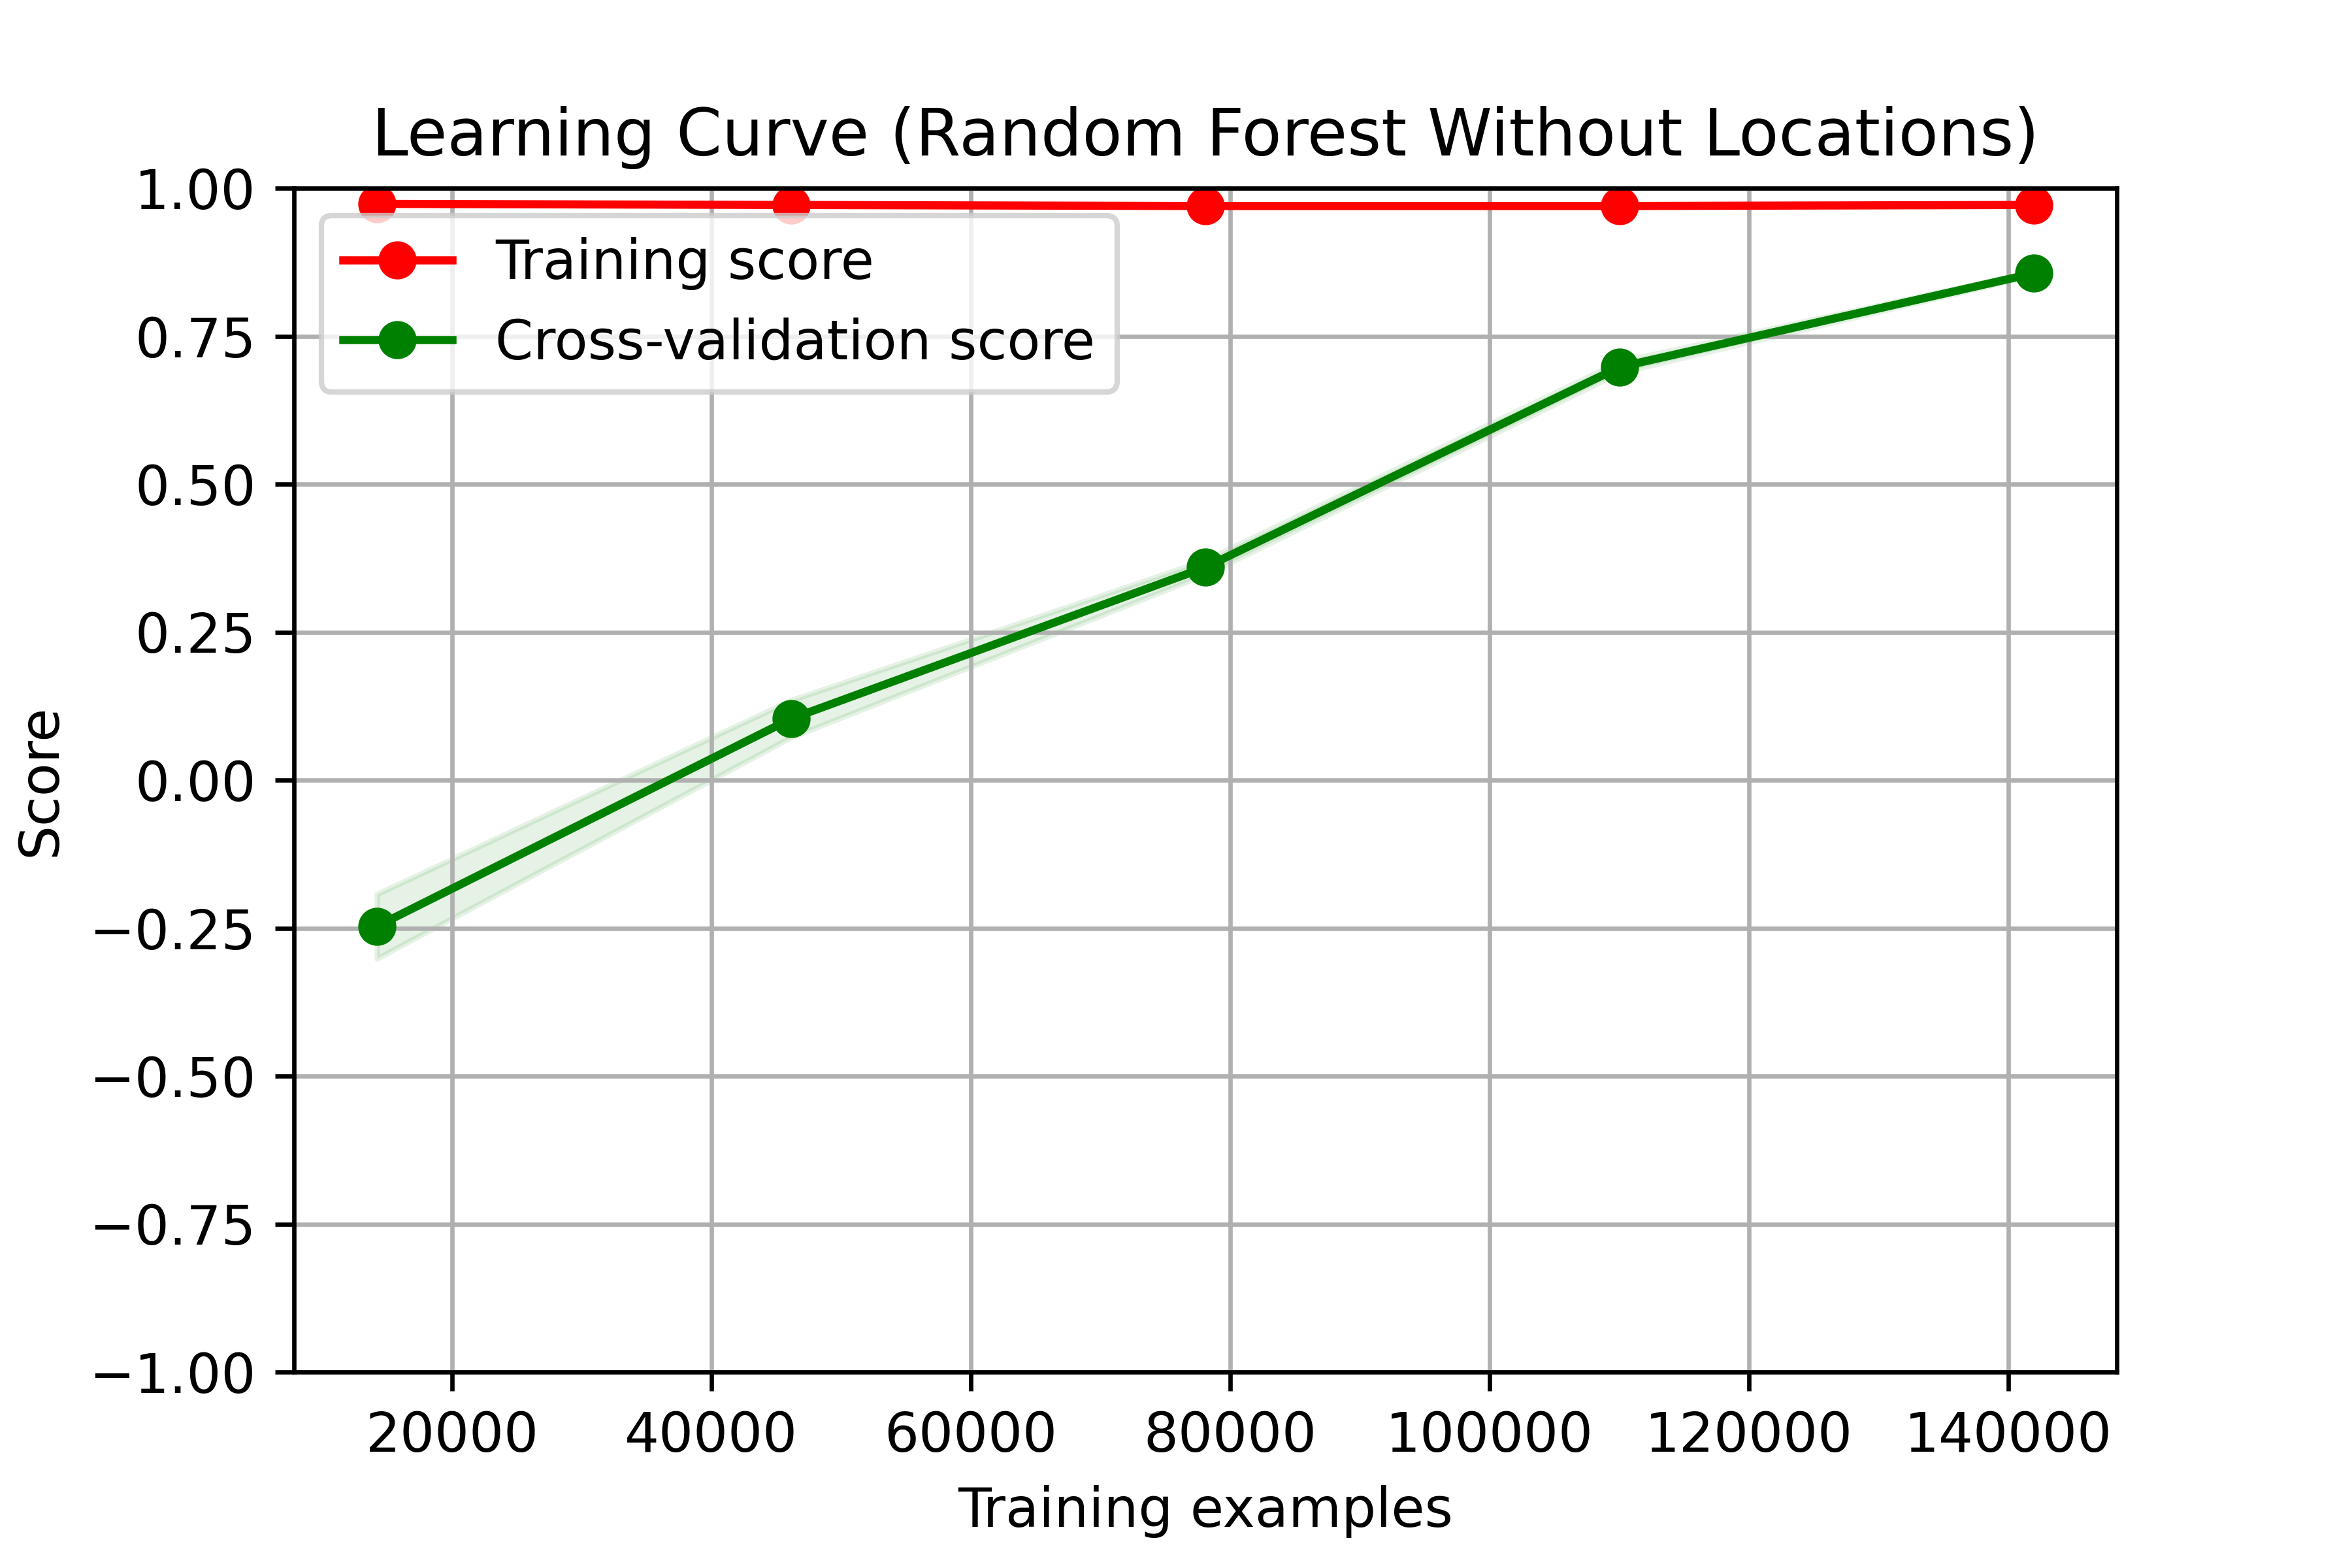
\includegraphics[width=0.5\linewidth]{./figures/Learing Curve1.png}}
  \subfloat{%
        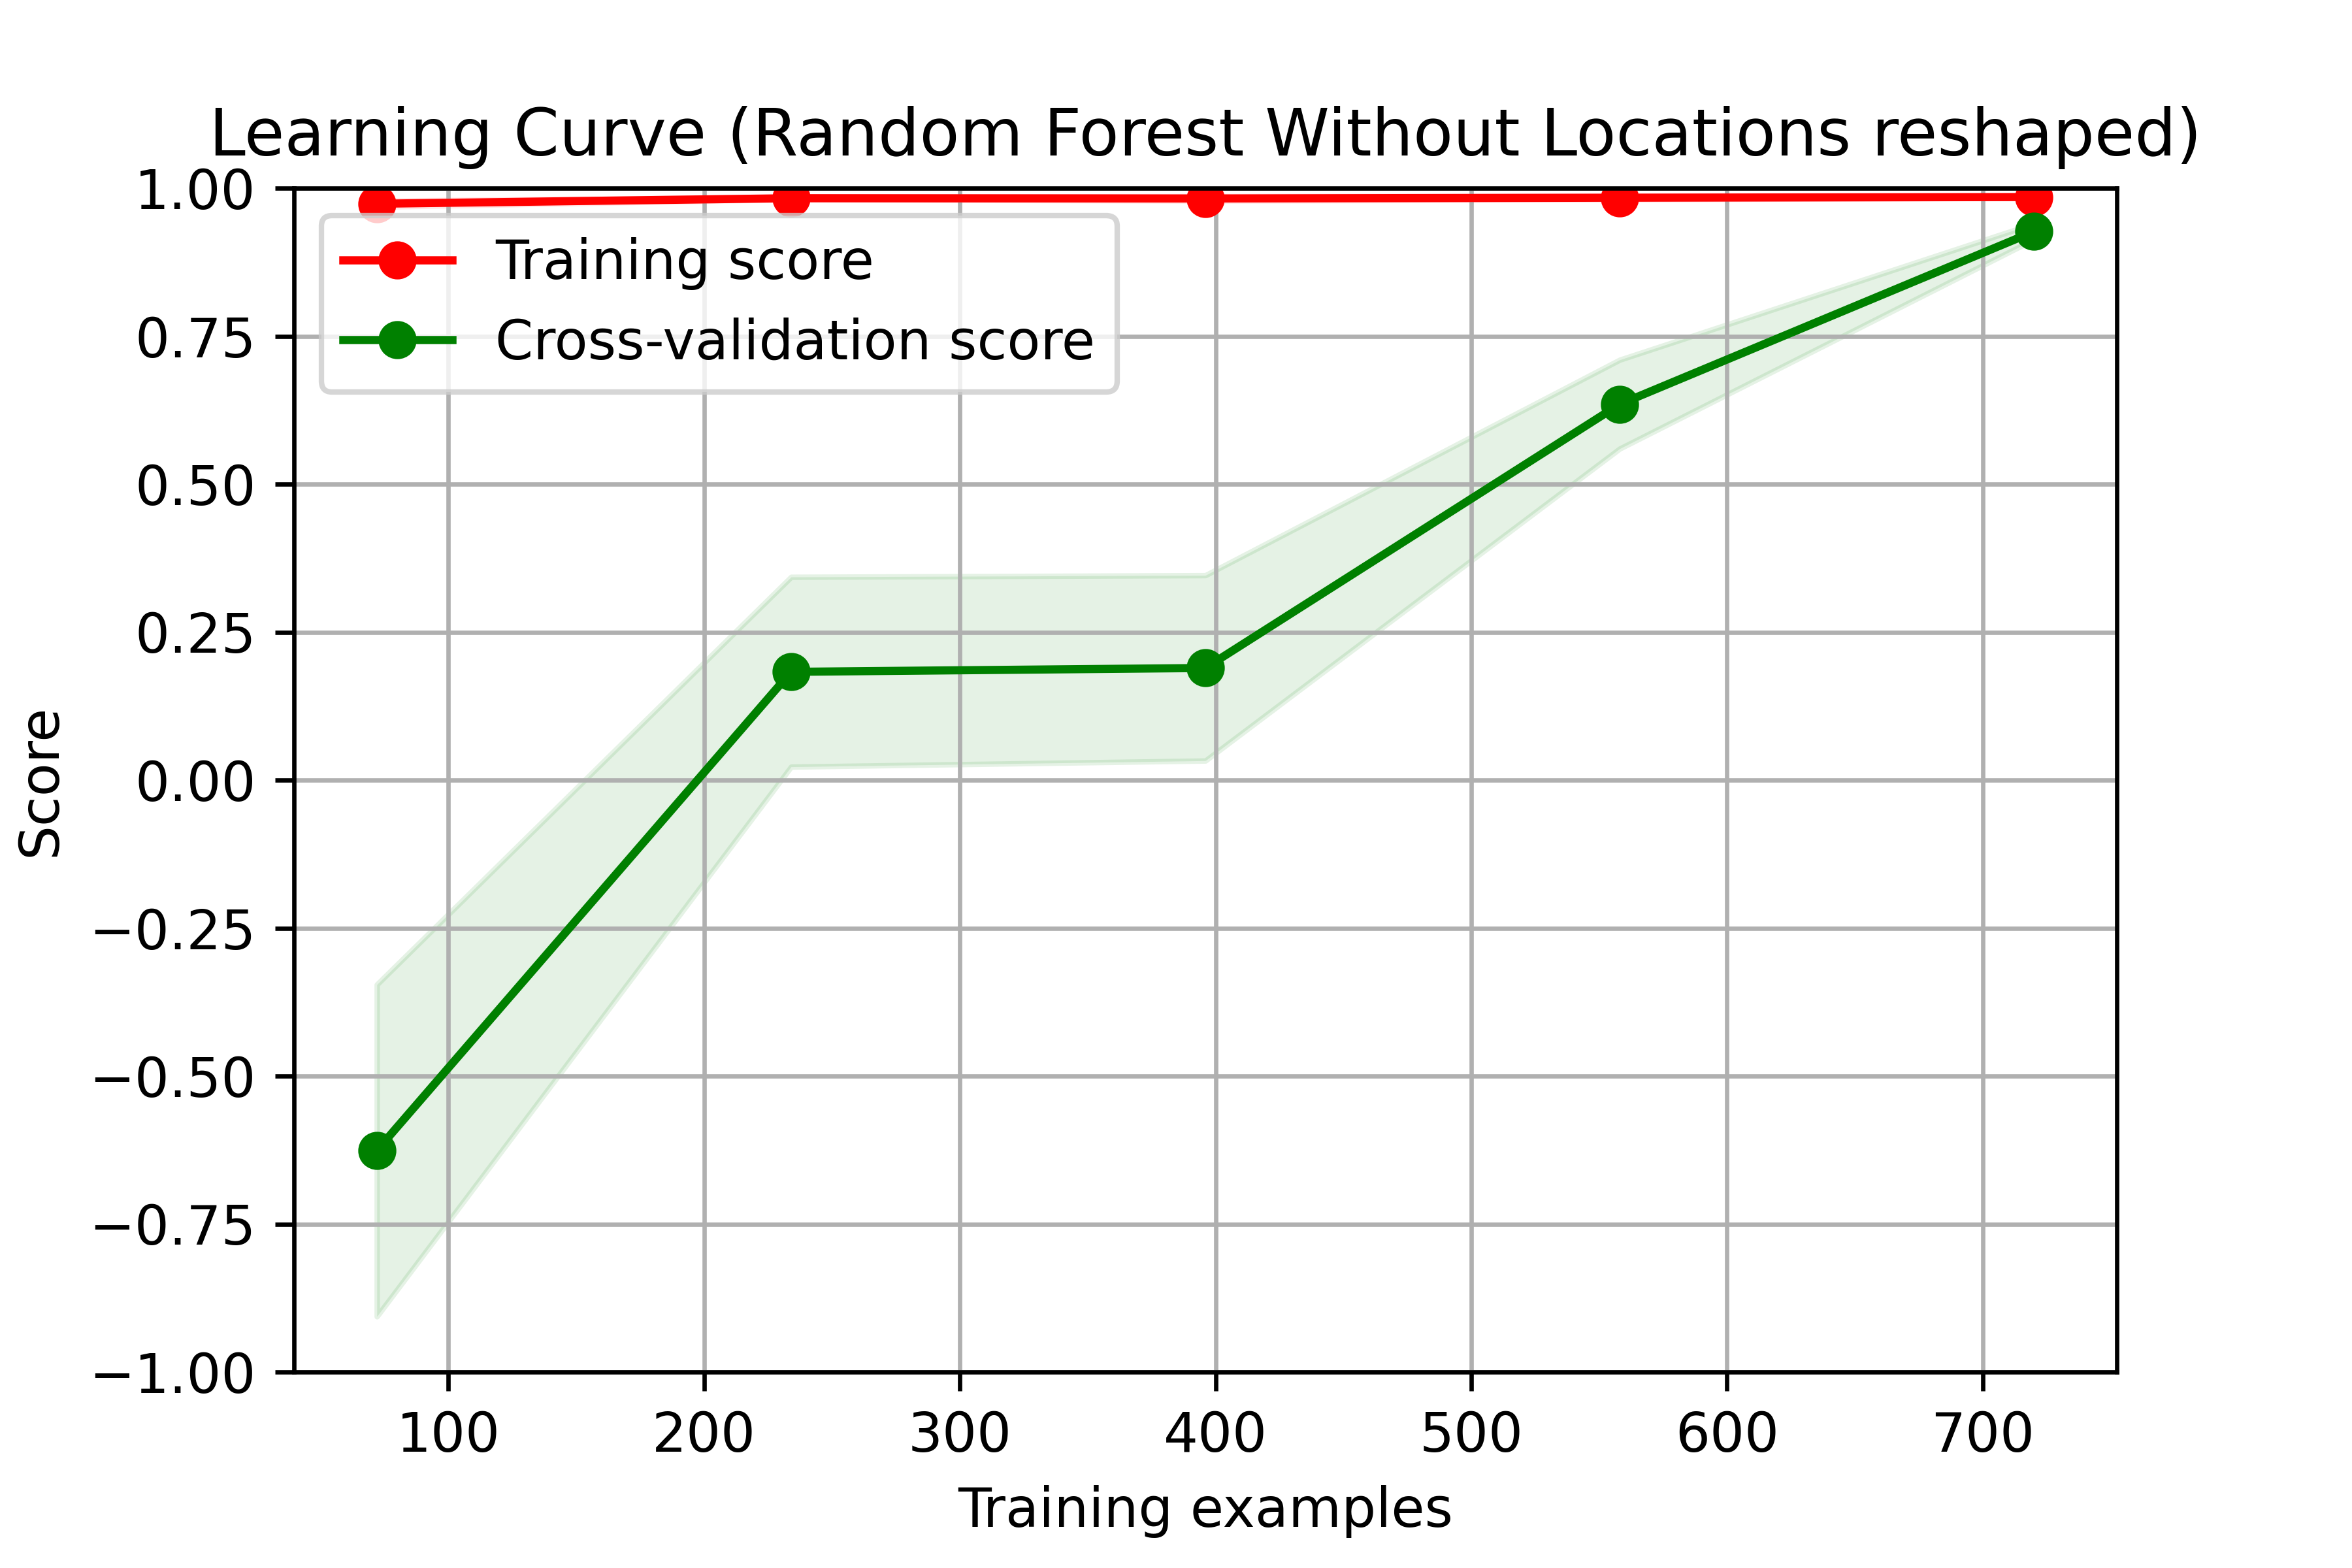
\includegraphics[width=0.5\linewidth]{./figures/Learing Curve2.png}}
  \hfill
  \subfloat{%
        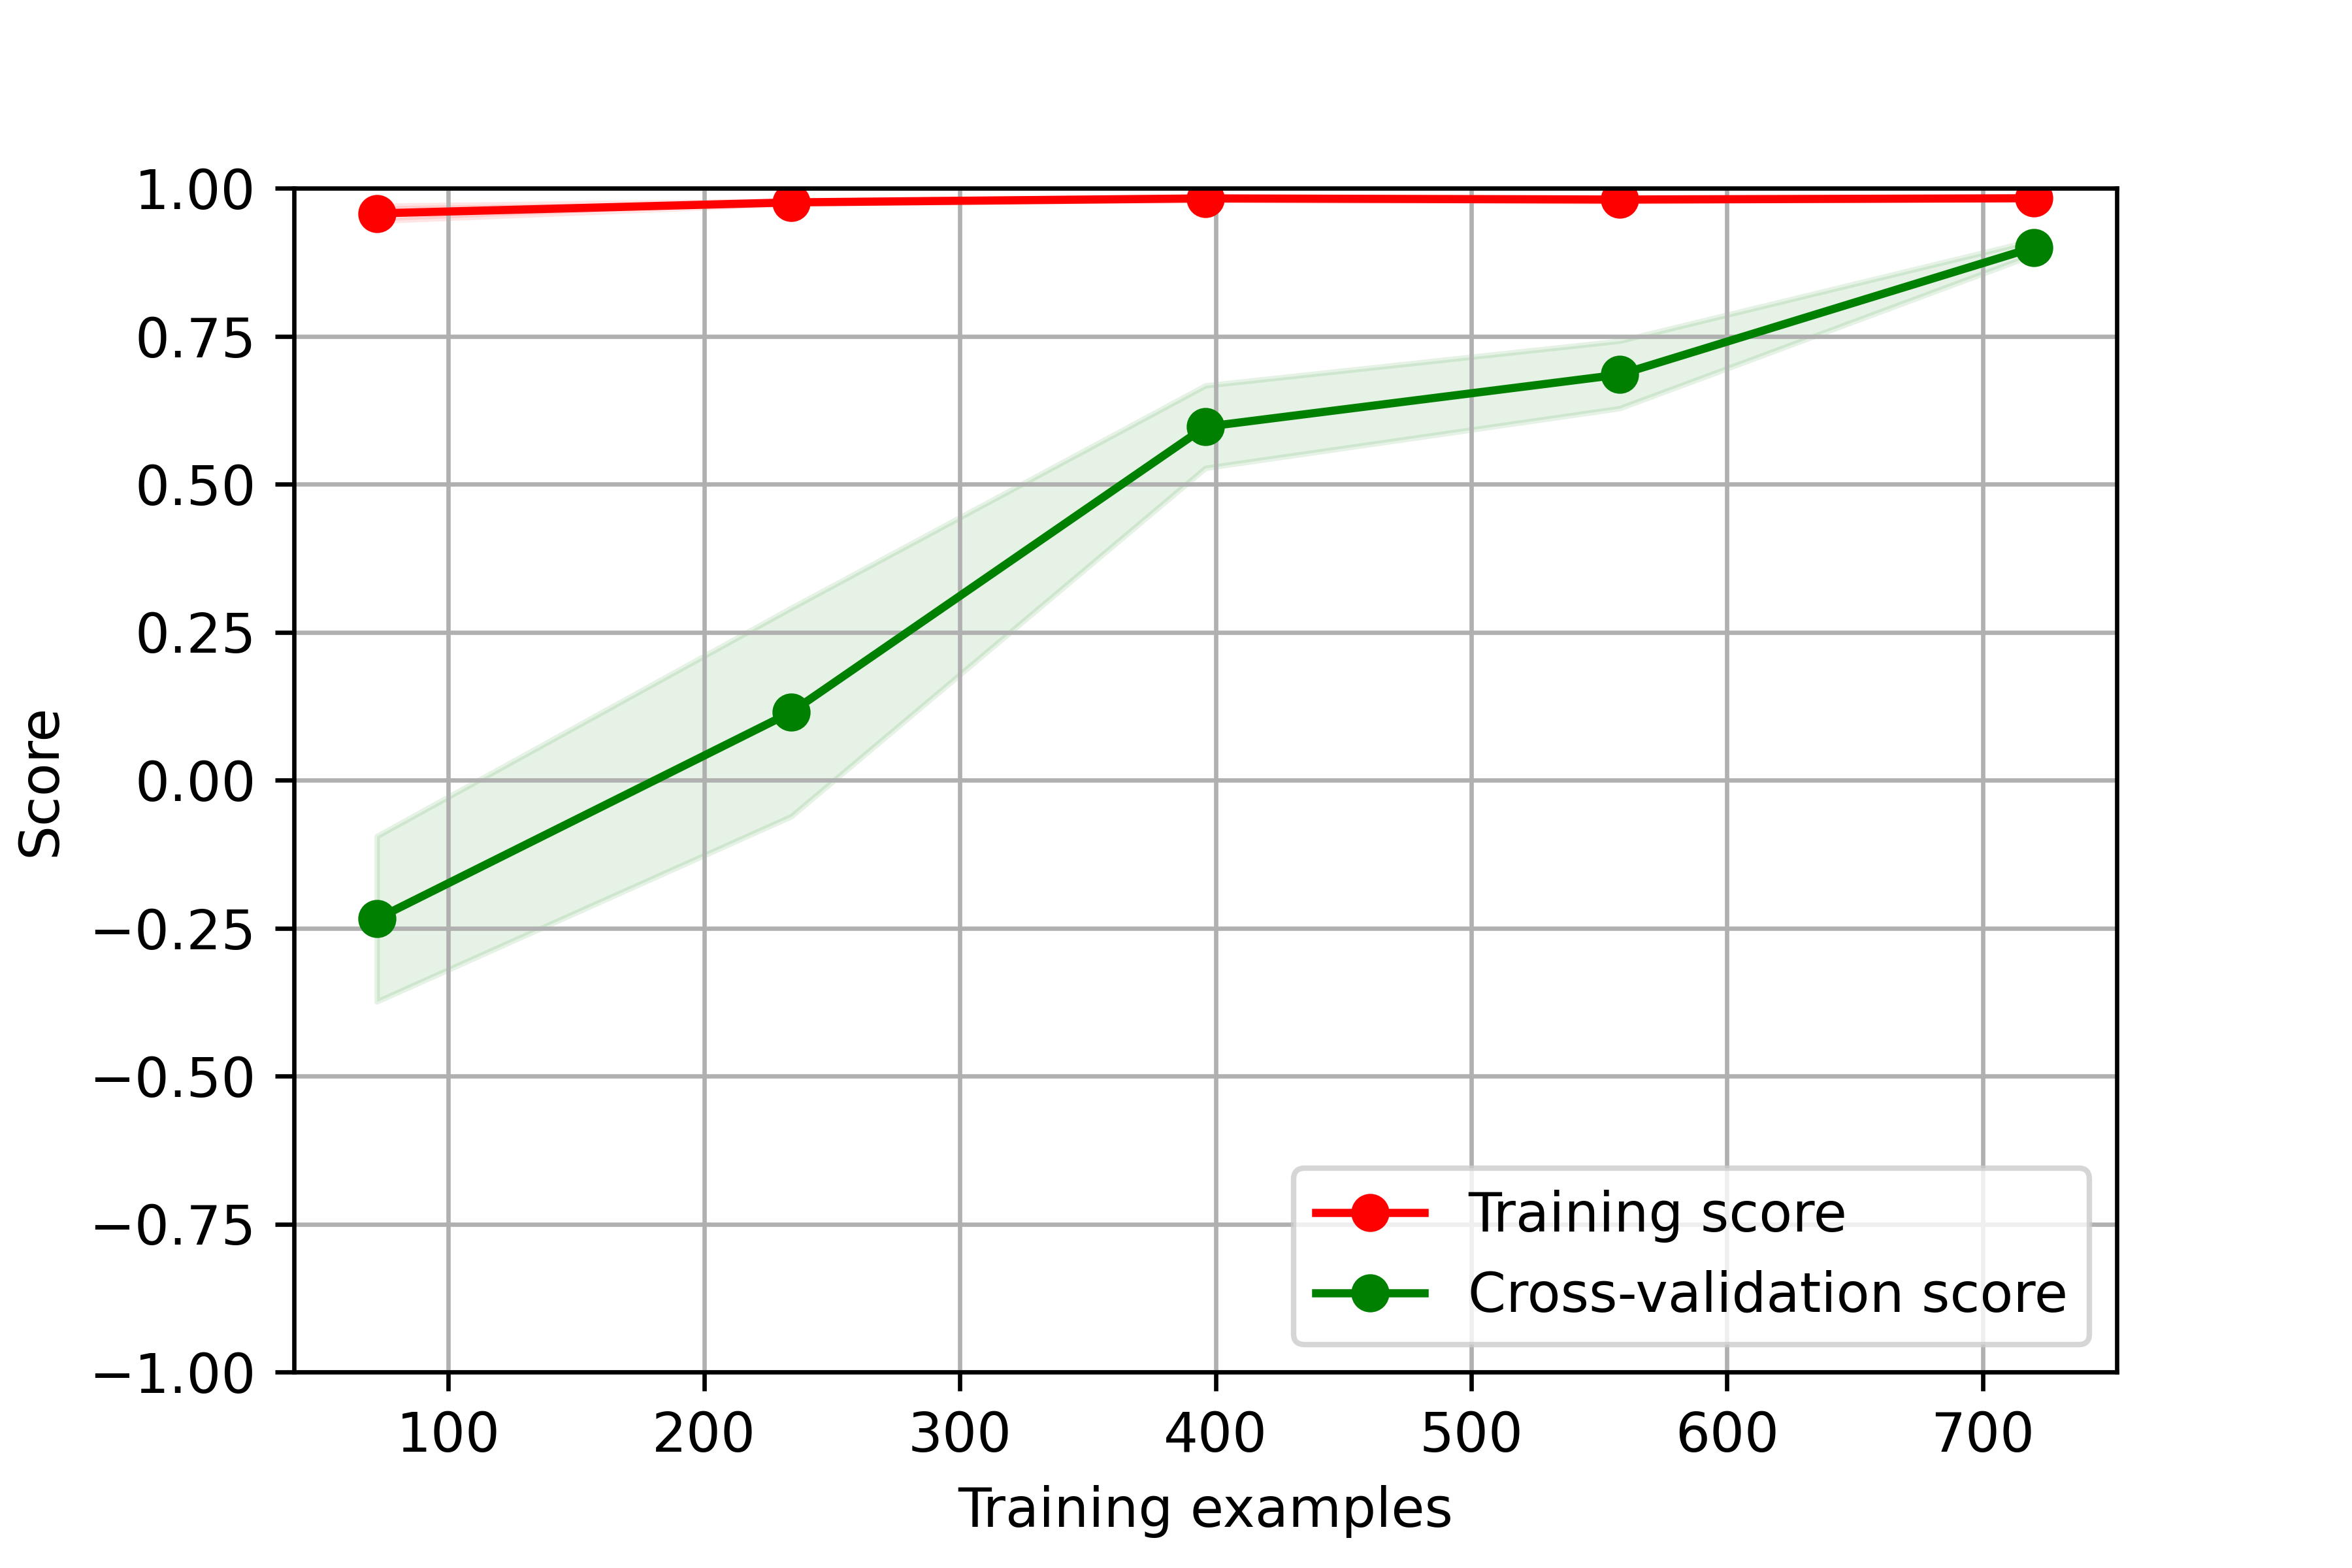
\includegraphics[width=0.5\linewidth]{./figures/Learing_Curve3.png}}
  \subfloat{%
        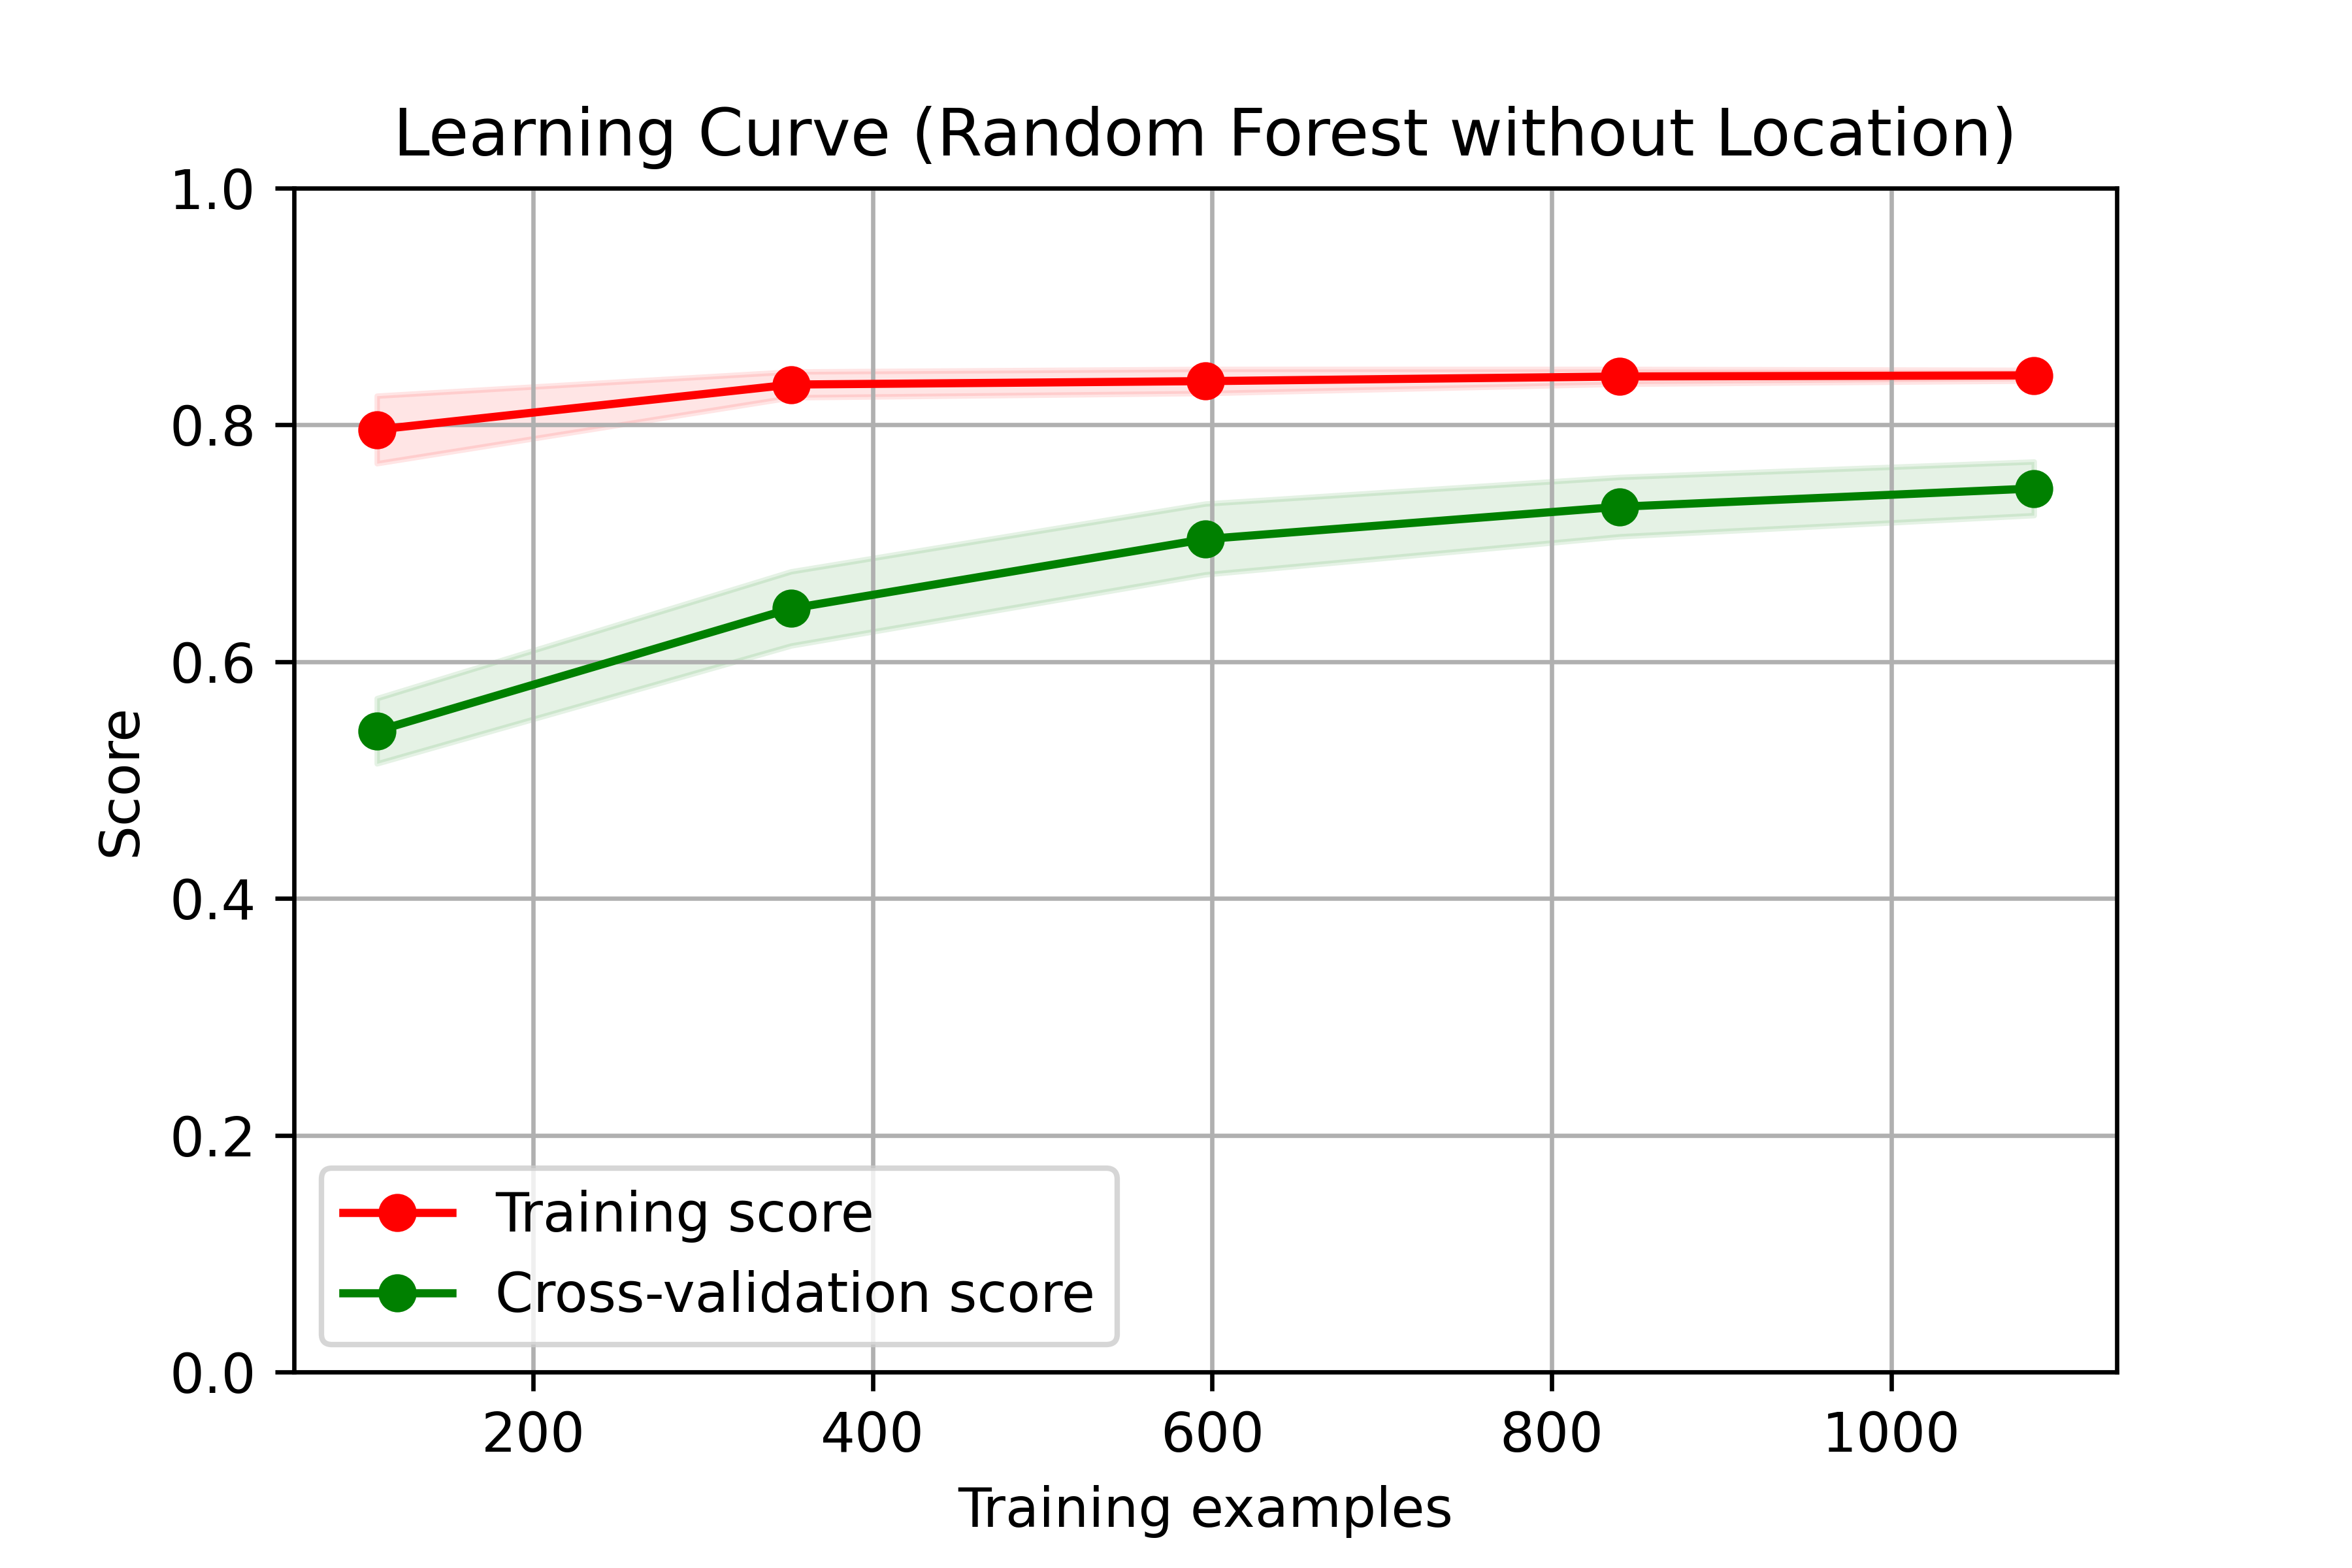
\includegraphics[width=0.5\linewidth]{./figures/cv4.png}}
    \caption{Learning Curve of Random Forest. (a) generated by the origin data, obviously, there's severe overfitting. (b) generated by setting data of different days to a new feature, performance gets worse. (c) generated by compress the data, the CV-score gets better. (d) generated by feature selection, the overfitting problem being solved}
    \label{fig:of}
  \end{figure}

  Go through the dataset, finding that the yield is bound to everyday log, which means that there are 186 different weather conditions with the same yield for every location. So we reshape the data to shrink the disparity in volume between yield and data entries. For data in 2013, the original shape is $(166685,16)$ (186 days $\times$ 901 locations,  16 features). Transform the shape of data into $(901\times2960)$ (901 locations, 185 days $\times$ 16 features) and run the test again. Learning curve of the result is shown in Fig.~\ref{fig:of}(b). These two methods can't solve the overfitting problem.

  Try to aggregate the data to shrink the number of features. Calculate the mean values of ever 60 days and shrink the number of features to 48 and run the test again. Learning curve of the results is shown in Fig.~\ref{fig:of}(c). There is some improvement after half of the dataset getting involved.

  To extract some indirect features from the origin features, we calculate the minimum and maximum value of features in 30 days, minimum maximum NDVI in 30 days, mean temperature difference, and variance e.t using a rolling window method from pandas. Then, run the test base on these features get the learning curve Fig.~\ref{fig:of}(d). The gap between training score and cross-validation score are narrowed, and improved the performance when 


\section{Conclusion and Future work} \label{sec:con}
  We composed a Bi-LSTM model with a CNN feature extraction sub-network to predict the wheat yield in the U.S and compared it with some commonly used regression algorithms and naive LSTM. The results show that the model outperforms the other algorithms and is less likely to get overfitting which is commonly found in other regression algorithms. Compare to the naive Bi-LSTM, the CNN feature extraction sub-network can help the Bi-LSTM fit the data better and reduce the disparity of performance between that on training set and test set.
  
  However, there are still some factors we do not consider due to the limitation of data. Some features crucial to crop growth, such as how farmers plant the crop and the condition of the sow in a certain location e.t, are not involved in the models due to the lack of data sources. The weather, undoubtedly, greatly influence the yield of corps, but some subjective behaviors of human can also influence the yield. The corps is not planted in an environment free of human intervention, water the crops when precipitation is a basic natural behavior that people influence the planting. If can get access such sort of data, the accuracy of prediction will be higher. 

\bibliographystyle{IEEEtran}
\bibliography{IEEEabrv,reference}

\end{document}
